\documentclass[a4paper,12pt]{article}

% --- Grundlegende Pakete ---
\usepackage[utf8]{inputenc}      % UTF-8 Eingabe
\usepackage[T1]{fontenc}         % Saubere Ausgabe
\usepackage[ngerman]{babel}      % Deutsche Sprache
\usepackage{lmodern}             % Moderne Schrift
\usepackage{microtype}           % Schönere Typografie

% --- Mathe & Symbole ---
\usepackage{amsmath, amssymb, amsthm}
\usepackage{dsfont}
\numberwithin{equation}{subsection}
\renewcommand{\theequation}{\thesubsection.\arabic{equation}}

% --- Layout & Struktur ---
\usepackage{geometry}
\geometry{margin=2.5cm}

\usepackage{setspace}            % Zeilenabstand
\onehalfspacing

\usepackage{parskip}             % Abstand zwischen Absätzen statt Einrückung

% --- Grafiken & Tabellen ---
\usepackage{graphicx}
\usepackage{float}
\usepackage{booktabs}
\usepackage{tikz}
\usepackage[compat=1.1.0]{tikz-feynman}

% --- Farben & Links ---
\usepackage{xcolor}
\usepackage[
    colorlinks=true,
    linkcolor=blue,
    urlcolor=blue,
    citecolor=blue
]{hyperref}

% --- Literatur (BibTeX) ---
\usepackage[numbers]{natbib}

% --- PDF ---
\usepackage{pdfpages}
\usepackage{xparse}

% --- Commands ---

\providecommand{\ket}[1]{\left|#1\right\rangle}
\providecommand{\bra}[1]{\left\langle#1\right|}
\providecommand{\erw}[1]{\left\langle#1\right\rangle}
\NewDocumentCommand{\lend}{m o}{\begin{flushright}
    #1\\[-0.8em]
    \rule{3cm}{0.4pt}
    \IfValueT{#2}{\\[-0.1em]#2}
  \end{flushright}}
\providecommand{\stp}[1]{\noindent\textbullet\ #1}

% Ueberschrift zwischen subsection und subsubsection, mit TOC-Eintrag
\newcounter{subsubmidsection}[subsection]
\renewcommand{\thesubsubmidsection}{\alph{subsubmidsection}}
\newcommand{\subsubmidsection}[1]{%
    \refstepcounter{subsubmidsection}%
    \addcontentsline{toc}{subsubsection}{\protect\numberline{\thesubsubmidsection\textup{)}}#1}%
    \par\vspace{0.75\baselineskip}%
    {\fontsize{13}{15.5}\selectfont\bfseries \thesubsubmidsection\textup{)}\quad #1\par}%
    \vspace{0.35\baselineskip}%
}
\newcommand{\icon}[2][3ex]{%
  \ensuremath{\mathord{\vcenter{\hbox{\includegraphics[height=#1]{Icon/#2}}}}}%
}


% --- Titelblatt infos ---
\newcommand{\todo}[1]{\textcolor{red}{TODO: #1}}
\newcommand{\vorlesungstitel}{Introduction to Feynman Diagrams and Quantum Field Theory with Applications to Solid State Physics}
\newcommand{\professor}{Prof. Dr. Frank Jahnke}
\newcommand{\mitschriftvon}{Bastian Koberg}

\begin{document}
\hypersetup{pageanchor=false}

\begin{titlepage}
  \centering
  \vspace*{3.5cm}
  {\Huge \textbf{\vorlesungstitel} \par}
  \vspace{1.2cm}
  {\Large Vorlesungsmitschrift \par}
  \vspace{1.8cm}
  {\large Dozent: \professor \par}
  \vspace{0.6cm}
  {\large Mitschrift: \mitschriftvon \par}
  \vfill
  {\large \today \par}
\end{titlepage}

\pagenumbering{roman}
\tableofcontents
\newpage
\hypersetup{pageanchor=true}
\pagenumbering{arabic}
\setcounter{page}{1}
\setcounter{tocdepth}{3} % Subsubsections im Inhaltsverzeichnis anzeigen

\section*{0. Motivation}

Vielteilchenproblem:
\begin{itemize}
    \item Praktisch unmöglich, Vielteilchen-Wellenfunktionen zu berechnen.
    \item Unendliche Hierarchie von Bewegungsgleichungen.
\end{itemize}

Lösung:
\begin{itemize}
    \item Neue Formulierung.
    \item Informationsüberschuss eliminieren.
\end{itemize}

\newpage
\providecommand{\ket}[1]{\left|#1\right\rangle}
\providecommand{\bra}[1]{\left\langle#1\right|}
\providecommand{\erw}[1]{\left\langle#1\right\rangle}
\providecommand{\lend}[1]{\begin{flushright}
#1\\[-0.8em]
\rule{3cm}{0.4pt}
\end{flushright}}

\section{Wechselwirkendes Elektronengas}

\subsection{Reduzierte Dichtematrizen und Propagatoren}

\subsubsection*{Reduzierte Dichtematrix}
Statistischer Operator:


\begin{equation}
\erw{A} = \mathrm{Sp}\{\varrho A\}
\end{equation}


für einen beliebigen Operator \(A\).  
Wir betrachten ein \(N\)-Teilchen-System.

Einteilchenoperator:

\begin{equation}
A = \sum_i A_i \quad
\raisebox{0.8ex}{$
\begin{array}[t]{l}
\text{\(A_i\) wirkt auf den Zustand}\\
\text{des \(i\)-ten Teilchens}
\end{array}
$}
\end{equation}

Wir benutzen die \(N\)-Teilchen-Basis:
\begin{equation}
\mathds{1} = \int dq_1 \dots dq_N \, \ket{q_1 \dots q_N}\bra{q_1 \dots q_N}
\end{equation}

\begin{center}
    $\hookrightarrow$ Vollständigkeitsrelation
\end{center}

Damit:


\begin{align}
\erw{A}
&= \int dq_1 \dots dq_N \bra{q_1 \dots q_N} \varrho A \ket{q_1 \dots q_N} \notag\\
&= \int dq_1 \dots dq_N \,\int dq_1' \dots dq_N' \,
\underbrace{\bra{q_1 \dots q_N} \varrho \ket{q_1' \dots q_N'}}_{\text{Dichtematrix}}
\underbrace{\bra{q_1' \dots q_N'} A \ket{q_1 \dots q_N}}_{\text{Matrixelement}} \notag\\
&= N \int dq_1 \dots dq_N \,\int dq_1' \dots dq_N'\,
\bra{q_1'}A_1\ket{q_1} \,
\underbrace{\bra{q_2' \dots q_N'} \ket{q_2 \dots q_N}}_{\delta_{ij} \text{(Orthogonalität der Basis)}}
\bra{q_1 \dots q_N} \varrho \ket{q_1' \dots q_N'} \notag\\
&= \int dq_1 \,\int dq_1' \, \bra{q_1'}A_1\ket{q_1} \, \varrho(q_1,q_1') \quad (*)
\\[0.4em]
\varrho(q_1,q_1')
&= N \int dq_2 \dots dq_N \, \bra{q_1,q_2,\dots,q_N} \varrho \ket{q_1',q_2,\dots,q_N} \notag\\
&= N\,\mathrm{Sp}_{2\dots N}\{\varrho\}
\end{align}

\begin{center}
    $\hookrightarrow$ reduzierte Einteilchen-Dichtematrix (Abspuren der vollen Dichtematrix)
\end{center}

$\Rightarrow$ Für die Berechnung von Einteilchenoperatoren bedarf es nur der Einteilchendichtematrix.
$\Rightarrow$ Vielteilchentheorie über reduzierte Dichtematrizen formulieren um den Informationsüberschuss zu beseitigen.

\subsubsection*{Feldoperatoren in 2. Quantisierung}
Man kann Operatoren auch durch Feldoperatoren 2. Quantisierung formulieren

\begin{equation}
A = \sum_{s,s'}\int d^3r \,\int d^3r'  \,
\bra{\vec r\,',s'} A \ket{\vec r,s} \, \psi^\dagger_{s'}(\vec r\,') \psi_s(\vec r)
\end{equation}

Mit dem statistischen Operator folgt für den Erwartungswert:


\begin{equation}
\erw{A} = \sum_{s,s'}
\int d^3r \, \int d^3r'\,
\bra{\vec r\,',s'} A \ket{\vec r,s} \,
\mathrm{Sp}\{\varrho \, \psi^\dagger_{s'}(\vec r\,',t)\psi_s(\vec r,t)\} \quad (**)
\end{equation}



Vergleich von (*) und (**) liefert die reduzierte Einteilchen-Dichtematrix in 2. Quantisierung:


\begin{equation}
\varrho_{ss'}(\vec r,\vec r\,';t) = 
\mathrm{Sp}\{\varrho \, \psi^\dagger_{s'}(\vec r\,',t)\psi_s(\vec r,t)\}
= \erw{\psi^\dagger_{s'}(\vec r\,',t)\psi_s(\vec r,t)}
\end{equation}



Die Diagonalelemente der reduzierten Einteilen-Dichtematrix ist der Erwartungswert der Teilchendichte


\begin{equation}
\erw{\varrho(\vec r,t)} = \sum _ s \varrho_{ss}(\vec r,\vec r)
\end{equation}


\subsubsection*{Propagatoren}

Zur Untersuchung der Bewegungsgleichung bilden die die Zeitableitung der reduzierten Dichtematrix:


\begin{equation}
 \frac{\partial}{\partial t} \varrho_{ss'}(\vec r,\vec r\,',t)
= \erw{\frac{\partial}{\partial t}\psi^\dagger_{s'}(\vec r\,',t)\,\psi_s(\vec r,t)
+ \psi^\dagger_{s'}(\vec r\,',t)\,\frac{\partial}{\partial t}\psi_s(\vec r,t)}
\end{equation}



Bisher: Heisenberg-Bewegungsgleichung für einzeitige Funktionen.  \\
Jetzt: zweizeitige Funktionen. Man setzt für ein t t' ein. Weil ohne Beschränkung der Allgemein kann man es so verallgemeinern.

\begin{equation}
\begin{aligned}
\label{propagatoren}
\erw{\psi^\dagger_s(\vec r,t)\psi_{s'}(\vec r\,',t')}
&= -i \hbar G^{<}_{ss'}(\vec r,t; \vec r\,',t')\\
\erw{\psi_s(\vec r,t)\psi^\dagger_{s'}(\vec r\,',t')}
&= i \hbar G^{>}_{ss'}(\vec r,t; \vec r\,',t')
\end{aligned}
\end{equation}



Das sind zwei verschiedene Größen da es keinen zweizeitgen Kommutator gibt, und sie also nicht so einfach zu vertauschen sind.\\
\\
Im Grundzustand $\ket{\phi_G}$ dann ist der statistische Operator der Projektionsoperator $\varrho = \ket{\phi_G}\bra{\phi_G}$




\begin{equation}
\begin{aligned}
\erw{A}
= \mathrm{Sp}\{\varrho A\}
&= \sum_i \bra{i}\ket{\phi_G}\bra{\phi_G} A_i\ket{i}\\
&= \sum_i \bra{\phi_G} A_i\ket{i}\bra{i}\ket{\phi_G}\\
&= \bra{\phi_G} A\ket{\phi_G}
\end{aligned}
\end{equation}



Für $G^{>}$ folgt im Zustand $\ket{\phi_G}$:


\begin{equation}
\begin{aligned}
i\,G^{>}_{ss'}(\vec r,t; \vec r\,',t')
= \bra{\phi_G}
\underbrace{\psi_s(\vec r,t)}_{\substack{\text{Vernichtung }e^-\\\text{mit }s\text{ bei }\vec r,t}}
\underbrace{\psi^\dagger_{s'}(\vec r\,',t')}_{\substack{\text{Erzeugung }e^-\\\text{mit }s'\text{ bei }\vec r\,',t'}}
\ket{\phi_G},
\qquad t>t'
\end{aligned}
\end{equation}



Interpretation:  
Wahrscheinlichkeitsamplitude, dass ein Teilchen mit Spin s am Ort $\vec r$ zur Zeit $t$ erzeugt wird und darauf zur Zeit $t'$ ein Teilchen mit $s'$ an Stelle $\vec r\,'$ gefunden/vernichtet werden kann.

$\Rightarrow$ Elektronenpropagator für den Grundzustand

Analoge Anschauungen gelten für die zweite Formel aus \ref{propagatoren} und damit den Lochpropagator

\begin{equation}
-i\hbar\,G^{<}_{ss'}(\vec r,t;\vec r\,',t')
= \bra{\phi_G}\,\psi^\dagger_{s'}(\vec r\,',t')\,\psi_s(\vec r,t)\,\ket{\phi_G},
\qquad t<t'
\end{equation}

\lend{Vorl. 10.04.2026}


\subsubsection*{Kompakte Schreibweise und zeitgeordnete Green-Funktionen}

Kompakte Schreibweise für die Argumente:

\begin{equation}
\bigl\{\vec r_1,t_1,s_1\bigr\} \equiv 1
\end{equation}

Im Heisenberg-Bild gilt damit kurz:

\begin{equation}
\psi_{s_1}(t_i) = \psi_{H,(1)}=\psi(1)
\end{equation}

Für die freie Green-Funktion schreibt man:

\begin{equation}
G^\gtrless_{s_1s_2}(\vec r_1,t_1;\vec r_2,t_2) = G^\gtrless (1,2)
\end{equation}

\subsubsection*{Kombination der Propagatoren zur Green-Funktion}

Da die beiden Propagatoren für unterschiedliche Zeitbereiche/Zeitfälle gelten, lassen sie sich zusammenfassen zu:

\begin{equation}
G(1,1') =
\begin{cases}
G^{>}(1,1') = -\frac{i}{\hbar}\,\erw{\psi(1)\psi^\dagger(1')}, & t_1 > t_1' \\
G^{<}(1,1') = \phantom{-}\frac{i}{\hbar}\,\erw{\psi^\dagger(1')\psi(1)}, & t_1 < t_1'
\end{cases}
\end{equation}

Alternative Schreibweise mit der Heaviside-Funktion \(\Theta(t)\):

\begin{equation}
G(1,1') = \Theta(t_1-t_1')\,G^{>}(1,1') + \Theta(t_1'-t_1)\,G^{<}(1,1')
\end{equation}

Der Zeitordnungsoperator \(T\) ordnet Feldoperatoren mit zunehmender Zeit nach links (late left). Für Fermionen entsteht bei jeder Vertauschung ein Minuszeichen. \(T\) hat nichts mit dem Kommutator zu tun, sondern wirkt nur bei ungleichen Zeiten.

\begin{equation}
G(1,1') = -\frac{i}{\hbar}\,\erw{T\,[\psi(1)\psi^\dagger(1')]}
\end{equation}


\subsubsection*{Eigenschaften/Informationen der GF}

Die Green-Funktion \(G\) heißt daher Einteilchen-zeitgeordnete (kausale) Green-Funktion.

\begin{itemize}
    \item Vorteile der Verwendung von \(G\)
    \begin{itemize}
        \item Feynman-Regeln für die systematische Berechnung von Green-Funktionen sind für die zeitgeordnete Green-Funktion am einfachsten.
    \end{itemize}
    \item Die Einteilchen-Green-Funktion enthält folgende Information:
    \begin{enumerate}
        \item Erwartungswerte von Einteilchenoperatoren
        \item Erwartungswert der Gesamtenergie \(\erw{H}\)
        \item Anregungsspektrum des Vielteilchensystems
    \end{enumerate}
\end{itemize}

\underline{1. Erwartungswert von Einteilchenoperatoren:}
\begin{equation}
A(t)=\sum_{s,s'}\int d^3r\,\int d^3r'\,\bra{\vec r\,',s'} A \ket{\vec r,s}\,\psi^{\dagger}_{s'}(\vec r\,',t)\,\psi_s(\vec r,t)
\end{equation}

Damit folgt fuer den Erwartungswert:

\begin{equation}
\erw{A}=\sum_{s,s'}\int d^3r\,\int d^3r'\,\bra{\vec r\,',s'} A \ket{\vec r,s}\,
\underbrace{\erw{\psi^{\dagger}_{s'}(\vec r\,',t)\psi_s(\vec r,t)}}_{-i\hbar\,G^{<}_{ss'}(\vec r,t;\vec r\,',t)}
\end{equation}

und mit der Vorschrift gleicher Zeiten als Grenzwert (
\(t_{+}=t+\varepsilon,\,\varepsilon\to 0, \varepsilon > 0\)):



Insbesondere fuer lokale Operatoren die nur an einem Ort wirken, also keine Uebergaenge $\vec r\to \vec r\,'$ mit $\vec r\neq \vec r\,'$ erzeugen.
Dadurch kollabiert der allgemeine Kernel auf einen Term proportional zu einer Deltafunktion.

\begin{equation}
\bra{\vec r\,',s'} A \ket{\vec r,s} = A_{s's}(\vec r)\,\delta(\vec r-\vec r\,')
\end{equation}

\begin{equation}
A(t)=\sum_{s,s'}\int d^3r\,\psi^{\dagger}_{s}(\vec r,t)\,A_{ss'}(\vec r)\,\psi_{s}(\vec r,t)
\end{equation}

\begin{equation}
\erw{A(t)}=\sum_{s,s'}\int d^3r\,\lim_{\vec r\,'\to \vec r}A_{ss'}(\vec r)\,\bigl[-i\hbar\,G_{s's}(\vec r,t;\vec r\,',t_{+})\bigr]
\end{equation}

Der Limes wird erst ausgefuehrt, nachdem der Operator auf die Green-Funktion angewendet wurde. Das wird gemacht damit A nur auf den linken Teil in der GF wirkt.

Beispiele:

\begin{equation}
\begin{aligned}
\erw{n(\vec r)}
&= \sum_s\erw{\psi^{\dagger}_s(\vec r,t)\psi_s(\vec r,t)}\\
&= -i\hbar\sum_s G_{ss}(\vec r,t;\vec r,t_{+})
\end{aligned}
\end{equation}

\begin{equation}
\begin{aligned}
\erw{T}
&= \sum_s\int d^3r\,\erw{\psi^{\dagger}_s(\vec r,t)\left(-\frac{\hbar^2}{2m}\Delta\right)\psi_s(\vec r,t)}\\
&= \sum_s\int d^3r\,\lim_{\vec r\,'\to \vec r}\left(-\frac{\hbar^2}{2m}\Delta_{\vec r}\right)\bigl[-i\hbar\,G_{ss}(\vec r,t;\vec r\,',t_{+})\bigr]
\end{aligned}
\end{equation}


\underline{2. Hamiltonoperator verwenden:}

\begin{equation}
\begin{aligned}
H
&= \sum_s\int d^3r\,\psi_s^{\dagger}(\vec r,t)\left(-\frac{\hbar^2}{2m}\Delta\right)\psi_s(\vec r,t)\\
&= \frac{1}{2}\sum_{s,s'}\int d^3r\,\int d^3r''\,\psi_s^{\dagger}(\vec r,t)\psi_{s'}^{\dagger}(\vec r\,'',t)\,V(\vec r-\vec r\,'')\,\psi_{s'}(\vec r\,'',t)\psi_s(\vec r,t)
\end{aligned}
\end{equation}

Zur Formulierung der Heisenberg-Bewegungsgleichung:

\begin{equation}
\begin{aligned}
i\hbar\,\frac{\partial}{\partial t}\psi_s(\vec r,t)
&= -\frac{\hbar^2}{2m}\Delta\,\psi_s(\vec r,t)\\
&\quad + \sum_{s''}\int d^3r''\,\psi_{s''}^{\dagger}(\vec r\,'',t)\,V(\vec r-\vec r\,'')\,\psi_{s''}(\vec r\,'',t)\psi_s(\vec r,t)
\end{aligned}
\end{equation}

Multipliziere von links mit $\psi_{s\,'}^{\dagger}(\vec r\,',t')$ und bilde den Erwartungswert:

\begin{equation}
\begin{aligned}
    \label{Heisenberg_Erwartungswert}
\left(i\hbar\frac{\partial}{\partial t}+\frac{\hbar^2}{2m}\Delta\right)\erw{\psi_{s\,'}^{\dagger}(\vec r\,',t')\psi_s(\vec r,t)}
&= \sum_{s''}\int d^3r''\,\erw{\psi_{s\,'}^{\dagger}(\vec r\,',t')\psi_{s''}^{\dagger}(\vec r\,'',t)\,V(\vec r-\vec r\,'')\,\psi_{s''}(\vec r\,'',t)\psi_s(\vec r,t)}
\end{aligned}
\end{equation}

Potentialenergie:

\begin{equation}
\begin{aligned}
\erw{V}
&= \frac{1}{2}\sum_{s,s''}\int d^3r\,\int d^3r''\,\psi_s^{\dagger}(\vec r,t)\psi_{s''}^{\dagger}(\vec r\,'',t)\,V(\vec r-\vec r\,'')\,\psi_{s''}(\vec r\,'',t)\psi_s(\vec r,t)\\
&= \frac{1}{2}\sum_s\int d^3r\,\lim_{\substack{\vec r\,'\to\vec r\\ t'\to t}}\left(i\hbar\frac{\partial}{\partial t}+\frac{\hbar^2}{2m}\Delta\right)\erw{\psi_s^{\dagger}(\vec r\,',t')\psi_s(\vec r,t)}\\
&= -\frac{i\hbar}{2}\sum_s\int d^3r\,\lim_{\substack{\vec r\,'\to\vec r\\ t'\to t_{+}}}\left(i\hbar\frac{\partial}{\partial t}+\frac{\hbar^2}{2m}\Delta\right)G_{ss}(\vec r,t;\vec r\,',t'_+)
\end{aligned}
\end{equation}

Um von Zeile 1 auf Zeile 2 zu kommen benutzt man Formel: \ref{Heisenberg_Erwartungswert}.  Ausdruck in der 1. Zeile ist bis auf den Faktor $\frac{1}{2}\sum\limits_s \int d^3r$ sowie die Bedingung $t'=t$ identisch mit dem Ausdruck aus der Bewegungsgleichung oben.

Das zusaetzliche $t'$ dient nur dazu, dass $\partial_t$ ausschliesslich auf $\psi_s(\vec r,t)$ wirkt und nicht auf $\psi_{s\,'}^{\dagger}(\vec r\,',t')$. Das ist dieselbe Begründung wie für das $\vec r'$

Zusammen folgt:

\begin{equation}
\begin{aligned}
\erw{H}
&= \erw{T}+\erw{V}\\
&= -\frac{i\hbar}{2}\sum_s\int d^3r\,\lim_{\substack{\vec r\,'\to\vec r\\ t'\to t_{+}}}\left(i\hbar\frac{\partial}{\partial t}-\frac{\hbar^2}{2m}\Delta\right)G_{ss}(\vec r,t;\vec r\,',t')
\end{aligned}
\end{equation}
3. Folgt im nächsten Abschnitt 

\lend{Vorl. 13.04.2026}
\subsection[Verschiedene GF und ihre Eigenschaften im thermodynamischen Gleichgewicht]{Verschiedene GF und ihre Eigenschaften}

\subsubsection*{Beschreibung von Propagatoren}

Die Betrachtung ist für ein system im thermodynamischen Gleichgewicht allerdings nicht bei $T=0\equiv$Grundzustand.

\stp{Erwartungswert: $\erw{\dots} = \mathrm{Sp}\!\left\{\varrho\,\dots \right\}$}

\stp{Statistischer Operator: $\varrho = \frac{e^{-\beta( H-\mu N)}}{\mathcal Z}$}

\stp{Zustandssumme: $\mathcal Z = \mathrm{Sp}\!\left\{e^{-\beta( H-\mu N)}\right\}$}

Da hier Operatoren zeitabhängig sind, sind sie im Heisenberg-Bild; $_H$ weggelassen.

\stp{Propagatoren und Green-Funktionen:}
\begin{align}
    G^{>}(1,1\mkern1mu') & = -\frac{i}{\hbar}\,\erw{\psi(1)\psi^{\dagger}(1\mkern1mu')},                 \\
    G^{<}(1,1\mkern1mu') & = +\frac{i}{\hbar}\,\erw{\psi^{\dagger}(1\mkern1mu')\psi(1)},                 \\
    G(1,1\mkern1mu')     & = -\frac{i}{\hbar}\,\erw{T\!\left[\psi(1)\psi^{\dagger}(1\mkern1mu')\right]}.
\end{align}

\stp{Vollständiger Satz von Eigenfunktionen:}
\begin{equation}
    \mathds{1} = \sum_n \ket{\Phi_n}\bra{\Phi_n},
\end{equation}
und
\begin{equation}
    H\ket{\Phi_n}=E_n\ket{\Phi_n},\qquad
    N\ket{\Phi_n}=N_n\ket{\Phi_n}
\end{equation}
folgt
\begin{align}
    G^{>}(1,1\mkern1mu')
     & = -\frac{i}{\hbar}\sum_n\bra{\Phi_n}\varrho\,\psi(1)\,\psi^{\dagger}(1\mkern1mu')\ket{\Phi_n}                         \\
     & = -\frac{i}{\hbar}\sum_n\bra{\Phi_n}\varrho\,\mathds{1}\,\psi(1)\,\mathds{1}\,\psi^{\dagger}(1\mkern1mu')\ket{\Phi_n} \\
     & = -\frac{i}{\hbar}\sum_{n,m}
    \underbrace{\bra{\Phi_n}\varrho\ket{\Phi_n}}_{\underbrace{e^{\beta(\Omega-E_n+\mu N_n)}}_{\omega_n} \delta_{nl}}
    \bra{\Phi_n}\psi(1)\ket{\Phi_m}
    \bra{\Phi_m}\psi^{\dagger}(1\mkern1mu')\ket{\Phi_n},
\end{align}

\stp{Für Heisenberg Operatoren gilt:}

\begin{align}
    \psi(1)                     & = e^{\frac{i}{\hbar}Ht_1}\,\psi_{s_1}(\vec r_1)\,e^{-\frac{i}{\hbar}Ht_1},                                                   \\
    \psi^{\dagger}(1\mkern1mu') & = e^{\frac{i}{\hbar}Ht_1\mkern1mu'}\,\psi^{\dagger}_{s_1\mkern1mu'}(\vec r_1\mkern1mu')\,e^{-\frac{i}{\hbar}Ht_1\mkern1mu'}.
\end{align}

Daraus folgt:

\begin{align}
    \label{eq:G_tdiff}
    G^{>}(1,1\mkern1mu')
     & = -\frac{i}{\hbar}\sum_{m,n}\omega_n\,
    \bra{\Phi_n}\psi_{s_1}(\vec r_1)\ket{\Phi_m}
    \bra{\Phi_m}\psi^{\dagger}_{s_1\mkern1mu'}(\vec r_1\mkern1mu')\ket{\Phi_n}
    e^{\frac{i}{\hbar}(E_n-E_m)(t_1-t_1\mkern1mu')},                       \\
    G^{<}(1,1\mkern1mu')
     & = \frac{i}{\hbar}\sum_{m,n}\omega_n\,
    \bra{\Phi_n}\psi^{\dagger}_{s_1\mkern1mu'}(\vec r_1\mkern1mu')\ket{\Phi_m}
    \bra{\Phi_m}\psi_{s_1}(\vec r_1)\ket{\Phi_n}
    e^{-\frac{i}{\hbar}(E_n-E_m)(t_1-t_1\mkern1mu')}                       \\
     & \overset{m\leftrightarrow n}{=} \frac{i}{\hbar}\sum_{m,n}\omega_m\,
    \bra{\Phi_n}\psi_{s_1}(\vec r_1)\ket{\Phi_m}
    \bra{\Phi_m}\psi^{\dagger}_{s_1\mkern1mu'}(\vec r_1\mkern1mu')\ket{\Phi_n}
    e^{\frac{i}{\hbar}(E_n-E_m)(t_1-t_1\mkern1mu')}.
\end{align}

Aus den Matrixelementen $\bra{\Phi_m}\psi^{\dagger}\ket{\Phi_n}$ und $\bra{\Phi_n}\psi\ket{\Phi_m}$ folgt $N_m=N_n+1$. Das folgt, da nachdem bspw. $\psi^\dagger$ auf $\ket{\Phi_n}$ angewandt wurde, müssen der neue Zustand und $\Phi_m$ dieselbe Anzahl an Teilchen haben. Ansonsten ist $\bra{\Phi_m}\psi^\dagger \ket{\Phi_n} = 0$. Daraus folgt:

\begin{align}
    \omega_m
     & = e^{\beta(\Omega-E_m+\mu N_m)}                                                \\
     & = e^{\beta(\Omega-E_n+\mu N_n)}\,e^{-\beta\left[(E_m-E_n)+\mu(N_m-N_n)\right]} \\
     & = e^{\beta(\Omega-E_n+\mu N_n)}\,e^{-\beta\left[(E_m-E_n)+\mu\right]}
\end{align}

\stp{Fouriertransformierte Propagatoren:}
Allgemein gilt die Fouriertransformation:
\begin{equation}
    G^{\gtrless}(\omega)
    = \int_{-\infty}^{\infty} d(t_1-t_1\mkern1mu')\,e^{i\omega(t_1-t_1\mkern1mu')}\,G^{\gtrless}(t_1-t_1\mkern1mu').
\end{equation}
Wir schreiben $G^{\gtrless}(t_1-t_1\mkern1mu')$, weil $G^{\gtrless}$ in der obigen Darstellung effektiv nur von $t_1-t_1\mkern1mu'$ abhängt.

Mit der Definition der Deltafunktion:

\begin{equation}
    \int_{-\infty}^{\infty} d(t_1-t_1\mkern1mu')\,
    e^{i\left(\omega-\frac{E_m-E_n}{\hbar}\right)(t_1-t_1\mkern1mu')}
    =2\pi\,\delta\!\left(\omega-\frac{E_m-E_n}{\hbar}\right).
\end{equation}

\begin{equation}
    \delta(ax)=\frac{1}{|a|}\,\delta(x).
\end{equation}

folgt die Fouriertransformierte:
\begin{equation}
    G^{\gtrless}(\omega)=\mp 2\pi i\sum_{m,n}\omega_n\,
    \underbrace{\left\{\begin{matrix}
            1 \\
            e^{-\beta(\hbar\omega-\mu)}
        \end{matrix}\right.}_{\substack{\text{Unterschied zwischen}\\ G^{>}\text{ und }G^{<}}}\,
    \erw{\dots}\,\erw{\dots}\,
    \delta\!\left(\hbar\omega-(E_m-E_n)\right).
\end{equation}

\subsubsection*{Spektralfunktion}

\begin{equation}
    \hat G(\omega)=G^{>}(\omega)-G^{<}(\omega)
\end{equation}
Ortsargumente sind hier nicht mitgeschrieben.

\stp{Im thermodynamischen Gleichgewicht gilt:}
\begin{equation}
    \hat G(\omega)
    =-2\pi i\sum_{m,n}\omega_n\left(1+e^{-\beta(\hbar\omega-\mu)}\right)
    \,\erw{\dots}\,\erw{\dots}\,
    \delta\!\left(\hbar\omega-(E_m-E_n)\right).
\end{equation}
Damit hat $\hat G(\omega)$ Peaks an den Übergangsenergien des Vielteilchensystems.

\stp{Zusammenhang zur Fermi-Funktion:}
\begin{equation}
    f(\omega)=\frac{1}{e^{\beta(\hbar\omega-\mu)}+1}
\end{equation}

\begin{equation}
    \hat G(\omega)=\left(1+e^{-\beta(\hbar\omega-\mu)}\right)G^{>}(\omega)
\end{equation}

Damit folgt im thermodynamischen Gleichgewicht (KMS-Relation):
\begin{align}
    G^{>}(\omega) & = \left[1-f(\omega)\right]\hat G(\omega), \\
    G^{<}(\omega) & = -f(\omega)\hat G(\omega).
\end{align}
$\Rightarrow$ Fluktuations-dissipations-Theorem

\stp{Normierung der Spektralfunktion}
Ausgehend vom zeitabhängigen Greenschen Funktional $G(\vec r_1,\vec r_1\mkern1mu';t_1-t_1\mkern1mu')$ führt eine Fourier-Transformation in der Zeit zum frequenzabhängigen Ausdruck $G(\vec r_1,\vec r_1\mkern1mu';\omega)$, der weiterhin im Ortsraum definiert ist. Erst durch eine zusätzliche Fourier-Transformation in der Ortsdifferenz $(\vec r_1-\vec r_1\mkern1mu')$ erhält man den impulsaufgelösten Greenschen Funktional $\hat G_{\vec k}(\omega)$. Damit beschreibt $\hat G(\vec r_1,\vec r_1\mkern1mu',\omega)$ lokale spektrale Eigenschaften, während $\hat G_{\vec k}(\omega)$ die energieabhängige Struktur eines Zustands mit Impuls $\vec k$ liefert.
\begin{align}
    \hat G(\vec r_1,\vec r_1\mkern1mu',\omega)
     & = G^{>}(\vec r_1,\vec r_1\mkern1mu',\omega)-G^{<}(\vec r_1,\vec r_1\mkern1mu',\omega) \\
     & = \int d(t_1-t_1\mkern1mu')\,e^{i\omega(t_1-t_1\mkern1mu')}
    \left(-\frac{i}{\hbar}\right)
    \bigl[\erw{\psi(\vec r_1,t_1)\psi^{\dagger}(\vec r_1\mkern1mu',t_1\mkern1mu')}+
        \erw{\psi^{\dagger}(\vec r_1\mkern1mu',t_1\mkern1mu')\psi(\vec r_1,t_1)}\bigr].
\end{align}

Daraus folgt die Normierung:
\begin{align}
    \int\frac{d\omega}{2\pi}\,\hat G(\vec r_1,\vec r_1\mkern1mu',\omega)
     & = \int d(t_1-t_1\mkern1mu')
    \underbrace{\int\frac{d\omega}{2\pi}e^{i\omega(t_1-t_1\mkern1mu')}}_{\delta(t_1-t_1\mkern1mu')}
    \left(-\frac{i}{\hbar}\right)\erw{\cdots}                                                  \\
     & = \left(-\frac{i}{\hbar}\right)
    \bigl[\erw{\psi(\vec r_1,t_1)\psi^{\dagger}(\vec r_1\mkern1mu',t_1)}+
        \erw{\psi^{\dagger}(\vec r_1\mkern1mu',t_1)\psi(\vec r_1,t_1)}\bigr]_{t=t_1\mkern1mu'} \\
     & = \left(-\frac{i}{\hbar}\right)\delta(\vec r_1-\vec r_1\mkern1mu').
\end{align}

Für die impulsaufgelöste Spektralfunktion gilts dann:
\begin{equation}
    \hat G_{\vec k}(\omega)=\int d^3(\vec r_1-\vec r_1\mkern1mu')\,e^{-i\vec k\cdot(\vec r_1-\vec r_1\mkern1mu')}\,\hat G(\vec r_1,\vec r_1\mkern1mu',\omega)
\end{equation}
\begin{equation}
    \int\frac{d\omega}{2\pi}\,i\hbar\,\hat G_{\vec k}(\omega)=1.
\end{equation}

Außerdem ergibt sich für die Zustandsdichte des wechselwirkenden Vielteilchensystems
\begin{equation}
    \varrho(\omega)=\int\frac{d^3\vec k}{{(2\pi)}^3}\,i\hbar\,\hat G_{\vec k}(\omega).
\end{equation}



\lend{Vorl. 17.04.2026}

\subsection{Green-Funktionen für freie Teilchen}

\subsubsection*{Hamiltonoperator und Heisenberg-Gleichung}

\stp{Betrachten Teilchen mit Spin $s$; dieser wird im Folgenden nicht mitgeschrieben.}

\stp{Hamiltonoperator:}
\begin{equation}
    H = \int d^3r\,\psi^{\dagger}(\vec r,t)\left(-\frac{\hbar^2}{2m}\Delta\right)\psi(\vec r,t).
\end{equation}

\stp{Heisenberg-Bewegungsgleichung für Feldoperatoren:}
\begin{equation}
    i\hbar\,\frac{\partial}{\partial t}\psi(\vec r,t)
    = \bigl[\psi(\vec r,t),H\bigr]
    = -\frac{\hbar^2}{2m}\Delta\,\psi(\vec r,t).
\end{equation}
\qquad $\hookrightarrow \psi$ ist Operator; $\Delta$ wirkt nicht direkt auf $\psi$

\subsubsection*{Darstellung der Feldoperatoren in der Basis ebener Wellen}

Die Entwicklung des Feldoperators in Basis ebener Wellen:
\begin{equation}
    \psi(\vec r,t)=\sum_{\vec k} a_{\vec k}(t)\,\varphi_{\vec k}(\vec r).
\end{equation}
Die Einteilchenfunktionen sind ein vollständiges Orthonormalsystem und erfüllen die freie Schrödinger-Gleichung:
\begin{equation}
    \left(-\frac{\hbar^2}{2m}\Delta\right)\varphi_{\vec k}(\vec r)=E_{\vec k}\,\varphi_{\vec k}(\vec r).
\end{equation}
Für ebene Wellen gilt:
\begin{equation}
    \varphi_{\vec k}(\vec r)=\frac{1}{\sqrt{V}}\,e^{i\vec k\cdot\vec r},
    \qquad
    E_{\vec k}=\frac{\hbar^2 k^2}{2m}.
\end{equation}
Einsetzen in die Heisenberg-Gleichung liefert:
\begin{equation}
    \label{f:zeitentwOperatoren}
    \begin{aligned}
        i\hbar\,\frac{\partial}{\partial t}\sum_{\vec k} a_{\vec k}(t)\,\varphi_{\vec k}(\vec r)
         & = \sum_{\vec k} E_{\vec k}\,a_{\vec k}(t)\,\varphi_{\vec k}(\vec r),                                         \\
        \Rightarrow\quad i\hbar\,\frac{\partial}{\partial t}a_{\vec k}(t)
         & = E_{\vec k}\,a_{\vec k}(t),                                                                                 \\
        \Rightarrow\quad \underbrace{a_{\vec k}(t)}_{\text{Operator}}
         & = \underbrace{a_{\vec k}}_{\substack{\text{Operator}\\\text{zur Zeit }0}}\,e^{-\frac{i}{\hbar}E_{\vec k} t}.
    \end{aligned}
\end{equation}

\subsubsection*{Retardierte und avancierte GF}
\begin{equation}\label{f:BeginGra}
    \begin{aligned}
        G^{r,a}(1,1\mkern1mu')
         & = \pm\Theta\!\bigl(\pm(t_1-t_1\mkern1mu')\bigr)\left[G^{>}(1,1\mkern1mu')-G^{<}(1,1\mkern1mu')\right]                                                      \\
         & = \pm\Theta\!\bigl(\pm(t_1-t_1\mkern1mu')\bigr)\left(-\frac{i}{\hbar}\right)\,\erw{\psi(1)\psi^{\dagger}(1\mkern1mu')+\psi^{\dagger}(1\mkern1mu')\psi(1)}. \\
         & = \pm\Theta\!\bigl(\pm(t_1-t_1\mkern1mu')\bigr)\left(-\frac{i}{\hbar}\right)
        \sum_{\vec k,\vec k\mkern1mu'}
        \left[\erw{a_{\vec k}(t_1)a^{\dagger}_{\vec k\mkern1mu'}(t_1\mkern1mu')}+\erw{a^{\dagger}_{\vec k\mkern1mu'}(t_1\mkern1mu')a_{\vec k}(t_1)}\right]
        \frac{1}{V}e^{i(\vec k\cdot\vec r_1-i\vec k\mkern1mu'\cdot\vec r_1\mkern1mu')}
    \end{aligned}
\end{equation}

Räumlich homogenes System $\rightarrow$ es muss $G(\vec r,\vec r\mkern1mu')$ =  $G(\vec r-\vec r\mkern1mu')$ $\Rightarrow \erw{a_{\vec k}a^{\dagger}_{\vec k\mkern1mu'}}=\erw{a_{\vec k}a^{\dagger}_{\vec k}}\,\delta_{\vec k,\vec k\mkern1mu'}$\\
Sieht man in der Exponentialfunktion sehr gut. Bedeutet effektiv $\vec k = \vec k \mkern1mu'$
\begin{equation}
    G^{r,a}(1,1\mkern1mu')
    = \frac{1}{V}\sum_{\vec k}e^{i\vec k\cdot(\vec r_1-\vec r_1\mkern1mu')}
    G^{r,a}_{\vec k}(t_1,t_1\mkern1mu').
\end{equation}
mit
\begin{equation}
    G^{r,a}_{\vec k}(t_1,t_1\mkern1mu')
    = \pm\Theta\!\bigl(\pm(t_1-t_1\mkern1mu')\bigr)\left(-\frac{i}{\hbar}\right)
    \left[\erw{a_{\vec k}(t_1)a^{\dagger}_{\vec k}(t_1\mkern1mu')}+\erw{a^{\dagger}_{\vec k}(t_1\mkern1mu')a_{\vec k}(t_1)}\right].
\end{equation}

Mit der Zeitentwicklung der Operatoren (\autoref{f:zeitentwOperatoren}) folgt
\begin{equation}
    G^{r,a}_{\vec k}(t_1,t_1\mkern1mu')
    = \pm\Theta\!\bigl(\pm(t_1-t_1\mkern1mu')\bigr)\left(-\frac{i}{\hbar}\right)
    \underbrace{\erw{a_{\vec k}a^{\dagger}_{\vec k}+a^{\dagger}_{\vec k}a_{\vec k}}}_{=1\;\text{(Fermi-Antikommutator)}}
    e^{-\frac{i}{\hbar}E_{\vec k}(t_1,t_1\mkern1mu')}
\end{equation}
\begin{equation}
    \Rightarrow G^{r,a}_{\vec k}(t_1,t_1\mkern1mu') = G^{r,a}_{\vec k}(t_1-t_1\mkern1mu')
\end{equation}

Die Fourier-Transformation ähnlich wie bei der Lehman oben mit \autoref{f:FormelFürFourier}:
\begin{equation}
    \begin{aligned}
        G^{r,a}_{\vec k}(\omega) & =\int_{-\infty}^{\infty} d\tau\,e^{i\omega\tau}G^{r,a}_{\vec k}(\tau)                                                                                                               \\
                                 & = \in d\tau \frac{1}{2\pi i} \int d\omega\mkern1mu'\bigl(\mp\frac{i}{\hbar}\bigr)e^{i(\omega\pm\omega\mkern1mu'-\frac{E_{\vec k}}{\hbar})\tau} \frac{1}{\omega\mkern1mu'-i\epsilon} \\
                                 & = \mp \frac 1 \hbar \frac{1}{\mp \omega \pm \frac{E_{\vec k}}{\hbar} - i\epsilon }
    \end{aligned}
\end{equation}
liefert die Darstellung der retardierten und avancierten zeitgeordnete Gf im Frequenzraum
\begin{equation}
    G^{r}_{\vec k}(\omega)=\frac{1}{\hbar\omega-E_{\vec k}+i\varepsilon},
    \qquad
    G^{a}_{\vec k}(\omega)=\frac{1}{\hbar\omega-E_{\vec k}-i\varepsilon}.
\end{equation}

Damit liegt der Pol von $G^r_{\vec k}(\omega)$ bei der freien Einteilchenenergie $E_{\vec k}$ in der unteren Halbebene, während der entsprechende Pol von $G^a_{\vec k}(\omega)$ in der oberen Halbebene liegt. Diese analytische Struktur kodiert Kausalitaet und beschreibt im freien Fall ungedaempfte, scharf definierte Anregungen. Bei eingeschalteter Wechselwirkung wird die freie Energie in eine frequenzabhaengige, komplexe Quasiteilchenenergie $\tilde E_{\vec k}(\omega)$ umgeformt. Deren Realteil verschiebt die Lage des Pols (Energie- oder Bandenverschiebung), waehrend der Imaginaerteil eine endliche Linienbreite bzw. Daempfung erzeugt. Die Pole repraesentieren dann nicht mehr ideale freie Teilchen, sondern Quasiteilchen mit renormierter Energie und endlicher Lebensdauer.

\lend{Vorl. 20.04.2026}

\subsubsection*{Spectral Function}

Die Spektralfunktion ist durch die Differenz aus retardierter und avancierter Green-Funktion definiert:
\begin{equation}
    \hat G_{\vec k}(\omega)
    = G^r_{\vec k}(\omega)-G^a_{\vec k}(\omega)
    = 2i\,\mathrm{Im}\,G^r_{\vec k}(\omega).
\end{equation}
Mit der Dirac-Identitäet
\begin{equation}
    \frac{1}{x+i\varepsilon}=\mathcal P\frac{1}{x}-i\pi\delta(x)
\end{equation}
folgt für freie Teilchen unmittelbar
\begin{equation}
    \hat G_{\vec k}(\omega)=-2\pi i\,\delta(\hbar\omega-E_{\vec k}) = -\frac{2\pi i}{\hbar}\delta\left(\omega-\frac{E_{\vec k}}{\hbar}\right).
\end{equation}

\begin{figure}[h]
    \centering
    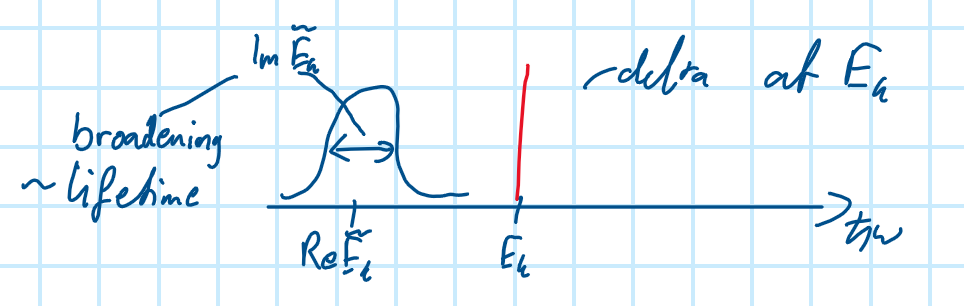
\includegraphics[width=0.78\linewidth]{Pictures/SpectralFunct.png}
    \caption{Skizze der Spektralfunktion: Im freien Fall liegt ein $\delta$-Peak bei $\hbar\omega=E_{\vec k}$ vor. Mit Wechselwirkung verschiebt sich das Maximum in Richtung $\mathrm{Re}\,\tilde E_{\vec k}$, und durch $\mathrm{Im}\,\tilde E_{\vec k}$ entsteht eine endliche Breite (Damping), die einer endlichen Lebensdauer der Quasiteilchen entspricht.}
    \label{fig:SpectralFunctionSketch}
\end{figure}

\subsubsection*{Propagators}

Für die Propagatoren gilt (analog zu \autoref{propagatoren}):
\begin{equation}
    G^{>}(1,1\mkern1mu')=-\frac{i}{\hbar}\,\langle\psi(1)\psi^{\dagger}(1\mkern1mu')\rangle,
    \qquad
    G^{<}(1,1\mkern1mu')=\frac{i}{\hbar}\,\langle\psi^{\dagger}(1\mkern1mu')\psi(1)\rangle.
\end{equation}
Analog zu der Berechnung von $G^{r,a}(1,1\mkern1mu')$ mit $a_{\vec k}(t)=a_{\vec k}e^{-\frac{i}{\hbar}E_{\vec k}t}$ (siehe Seite \pageref{f:BeginGra} und \autoref{f:zeitentwOperatoren}) folgt im Impulsraum
\begin{equation}
    G^{<}_{\vec k}(t_1,t_1\mkern1mu')
    = \frac{i}{\hbar}\,\langle a^{\dagger}_{\vec k}(t_1\mkern1mu')a_{\vec k}(t_1)\rangle
    = \frac{i}{\hbar}\,\langle a^{\dagger}_{\vec k}a_{\vec k}\rangle\,e^{-\frac{i}{\hbar}E_{\vec k}(t_1-t_1\mkern1mu')},
\end{equation}
\begin{equation}
    G^{>}_{\vec k}(t_1,t_1\mkern1mu')
    = -\frac{i}{\hbar}\,\langle a_{\vec k}(t_1)a^{\dagger}_{\vec k}(t_1\mkern1mu')\rangle
    = -\frac{i}{\hbar}\,\langle a_{\vec k}a^{\dagger}_{\vec k}\rangle\,e^{-\frac{i}{\hbar}E_{\vec k}(t_1-t_1\mkern1mu')}.
\end{equation}
Mit der Besetzungszahl $f_{\vec k}=\langle a^{\dagger}_{\vec k}a_{\vec k}\rangle$ und
$\langle a_{\vec k}a^{\dagger}_{\vec k}\rangle=1-f_{\vec k}$ erhaelt man nach Fourier-Transformation
\begin{equation}
    \begin{aligned}
        G^{\lessgtr}_{\vec k}(\omega)
         & = \int d\tau\,e^{i\omega\tau}G^{\lessgtr}_{\vec k}(\tau),
        \qquad \tau=t_1-t_1\mkern1mu',                                     \\
         & = \frac{i}{\hbar}
        \begin{Bmatrix}
            f_{\vec k} \\
            f_{\vec k}-1
        \end{Bmatrix}
        \int d\tau\,e^{i\left(\omega-\frac{E_{\vec k}}{\hbar}\right)\tau}, \\
         & = \frac{i}{\hbar}
        \begin{Bmatrix}
            f_{\vec k} \\
            f_{\vec k}-1
        \end{Bmatrix}
        \underbrace{2\pi\,\delta\!\left(\omega-\frac{E_{\vec k}}{\hbar}\right)}_{=i\hbar\,\hat G_{\vec k}(\omega)}.
    \end{aligned}
\end{equation}
und damit
\begin{equation}
    G^{<}_{\vec k}(\omega)=-f_{\vec k}\,\hat G_{\vec k}(\omega),
    \qquad
    G^{>}_{\vec k}(\omega)=(1-f_{\vec k})\,\hat G_{\vec k}(\omega).
\end{equation}

Damit enthält die Spektralfunktion die Information über die verfügbaren Zustaende, waehrend $f_{\vec k}$ deren Besetzung kodiert. Die Propagatoren $G^{<}$ und $G^{>}$ verknüpfen beide Informationen.
\newpage
\section{\texorpdfstring{Diagram-Methode für $T=0 \leftrightarrow$ Grundzustand}{Diagram-Methode für T=0 <-> Grundzustand}}
\subsection{Wechselwirkungs-Bild}

Wir zerlegen den Hamiltonoperator in
\begin{equation}
  H=H_0+H_{\mathrm{int}}.
\end{equation}
Dabei sei das Eigenwertproblem von $H_0$ lösbar.
Ziel ist es, den Einfluss von $H_{\mathrm{int}}$ systematisch zu beruecksichtigen.

\subsubsection*{Vergleich der Bilder}

\begin{center}
  \renewcommand{\arraystretch}{1.4}
  \begin{tabular}{@{}lll@{}}
    \toprule
    Bild         & Operatoren                                                                                                      & Wellenfunktion / Zustand                                                                    \\
    \midrule
    Schroedinger & $\dfrac{\partial}{\partial t}A_S=0$                                                                             & $i\hbar\,\dfrac{\partial}{\partial t}\ket{\phi_S(t)}=(H_0+H_{\mathrm{int}})\ket{\phi_S(t)}$ \\
    Heisenberg   & $A_H(t)=e^{\frac{i}{\hbar}(H_0+H_{\mathrm{int}})(t-t_0)}A_S\,e^{-\frac{i}{\hbar}(H_0+H_{\mathrm{int}})(t-t_0)}$ & $\dfrac{\partial}{\partial t}\ket{\phi_H}=0$                                                \\
    Interaction  & $A_0(t)=e^{\frac{i}{\hbar}H_0(t-t_0)}A_S\,e^{-\frac{i}{\hbar}H_0(t-t_0)}$                                       & $i\hbar\,\dfrac{\partial}{\partial t}\ket{\phi_0(t)}=H_{\mathrm{int}}^{(0)}\ket{\phi_0(t)}$ \\
    \bottomrule
  \end{tabular}
\end{center}

Zur Herleitung der Wellenfunktion im WW-Bild
benutzen wir die Picture-Unabhaengigkeit des
Erwartungswertes:
\begin{equation}
  \erw{A}
  =\bra{\phi_S(t)}A_S\ket{\phi_S(t)}
  =\underbrace{\bra{\phi_0(t)}}_{\text{Zustand im WW-Bild}}
  \,\underbrace{e^{\frac{i}{\hbar}
        H_0(t-t_0)}A_S\,e^{-\frac{i}{\hbar}H_0(t-t_0)}}_{\text{Operator }A_0(t)\text{ im WW-Bild}} \,\underbrace{\ket{\phi_0(t)}}_{\text{Zustand im WW-Bild}}.
\end{equation}
Dabei haben wir im Prinzip zwei Einsen eingefügt und benutzt, dass:
\begin{equation}
  \ket{\phi_0(t)}=e^{\frac{i}{\hbar}
      H_0(t-t_0)}\ket{\phi_S(t)}.
\end{equation}
Nun folgt die Bewegungsgleichung im WW-Bild direkt durch Ableiten:
\begin{equation}
  \begin{aligned}
    i\hbar\,\frac{\partial}{\partial t}\ket{\phi_0(t)}
     & = i\hbar\,\frac{\partial}{\partial t}\left(e^{\frac{i}{\hbar} H_0(t-t_0)}\ket{\phi_S(t)}\right)                                                  \\
     & = -H_0e^{\frac{i}{\hbar}H_0(t-t_0)}\ket{\phi_S(t)} +e^{\frac{i}{\hbar}H_0(t-t_0)}\left(i\hbar\,\frac{\partial}{\partial t}\ket{\phi_S(t)}\right) \\
     & = -H_0e^{\frac{i}{\hbar}H_0(t-t_0)}\ket{\phi_S(t)} +e^{\frac{i}{\hbar}H_0(t-t_0)}(H_0+H_{\mathrm{int}})\ket{\phi_S(t)}                           \\
     & = e^{\frac{i}{\hbar}H_0(t-t_0)}H_{\mathrm{int}}\ket{\phi_S(t)}                                                                                   \\
     & = e^{\frac{i}{\hbar}H_0(t-t_0)}H_{\mathrm{int}}e^{-\frac{i}{\hbar}H_0(t-t_0)}\ket{\phi_0(t)}                                                     \\
     & = \underbrace{e^{\frac{i}{\hbar}H_0(t-t_0)}H_{\mathrm{int}}e^{-\frac{i}{\hbar}H_0(t-t_0)}}_{\equiv\,H_{\mathrm{int}}^{(0)}(t)}\ket{\phi_0(t)}.
  \end{aligned}
\end{equation}
Genutzt wurde hier einmal die Schrödinger-Gleichung und der Fakt, dass $H_0$ mit sich selbst und mit sich selbst im Exponent $(e^{H_0})$ kommutiert.
Außerdem wurde erneut eine 1 eingefügt um aus dem Schrödinger-Zustand einen WW-Zustand zu machen.

Damit gilt asdf
\begin{equation}
  i\hbar\,\frac{\partial}{\partial t}\ket{\phi_0(t)}=H_{\mathrm{int}}^{(0)}(t)\ket{\phi_0(t)}.
\end{equation}
Hinweis: $H_0$ und $H_{\mathrm{int}}$ müssen dabei im Allgemeinen nicht kommutieren.

\subsubsection*{Formale Lösung der Bewegungsgleichung im WW-Bild}
\begin{equation}
  \label{eq:ww-eom}
  i\hbar\,\frac{\partial}{\partial t}\ket{\phi_0(t)}
  =H_{\mathrm{int}}^{(0)}(t)\ket{\phi_0(t)}.
\end{equation}
Fuer einen kleinen Zeitschritt $\delta t$:
\begin{equation}
  \begin{aligned}
    \ket{\phi_0(t+\delta t)} & = \ket{\phi_0(t)}+\delta\ket{\phi_0(t)}                                              \\
                             & =\ket{\phi_0(t)}-\frac{i}{\hbar}H_{\mathrm{int}}^{(0)}(t)\,\delta t\,\ket{\phi_0(t)} \\
                             & \approx e^{-\frac{i}{\hbar}H_{\mathrm{int}}^{(0)}(t)\,\delta t}\ket{\phi_0(t)}
    \qquad \text{Exponentialnaeerung für kleines }\delta t
  \end{aligned}
\end{equation}
Diese Allgemeine Formel können wir nun benutzen um das Intervall $[t_1,t_2]$ in vorerst endlich viele Teile Zeitintervalle $\delta t$ zu teilen.
Damit ist die gesamte Zeitentwicklung als Aneinanderreihung der $\delta t$ Zeitentwicklungen zu verstehen.
Die Zeitintervalle werden unendlich klein für eine exakte Darstellung.
\begin{equation}
  \begin{aligned}
    \ket{\phi_0(t_2)}
     & = \lim \limits_{\delta t \to 0}\cdots e^{-\frac{i}{\hbar}H_{\mathrm{int}}^{(0)}(t_{a})\delta t}e^{-\frac{i}{\hbar}H_{\mathrm{int}}^{(0)}(t_1)\delta t}\cdots\ket{\phi_0(t_1)}, \\
     & =\lim \limits_{\delta t \to 0}\mathcal T\prod_{t_i=t_1}^{t_2-\delta t}e^{-\frac{i}{\hbar}H_{\mathrm{int}}^{(0)}(t_i)\delta t}\ket{\phi_0(t_1)},
  \end{aligned}
\end{equation}
Nun ziehen wir das Produkt in die Exponentialfunktion als Summe und lassen $\delta t$ gegen 0 gehen, wodurch die Summe zu einem Integral wird.
Der Operator $\mathcal{T}$ sorgt für die richtige Zeitordnung der Exponentialfunktionen.
\begin{equation}
  \ket{\phi_0(t_2)}
  =\mathcal T\exp\!\left[-\frac{i}{\hbar}\int_{t_1}^{t_2}d\tau\,H_{\mathrm{int}}^{(0)}(\tau)\right]\ket{\phi_0(t_1)}.
\end{equation}
Schliesslich:
\begin{equation}
  \begin{aligned}
    \ket{\phi_0(t_2)}=S(t_2,t_1)\ket{\phi_0(t_1)}, \\
    S(t_2,t_1)=\mathcal T\exp\!\left[-\frac{i}{\hbar}\int_{t_1}^{t_2}d\tau\,H_{\mathrm{int}}^{(0)}(\tau)\right].
  \end{aligned}
\end{equation}

\lend{Vorl. 23.04.2026}

\subsubsection*{Eigenschaften der S-Operatoren}

\begin{equation}
  S(t_0,t)=\tilde{\mathcal T}\exp\!\left[\frac{i}{\hbar}\int_{t_0}^{t}d\tau\,H_{\mathrm{int}}^{(0)}(\tau)\right],
  \qquad t>t_0.
\end{equation}
Dabei laeuft der Operator in umgekehrter Zeitordnung, also rueckwaerts in der Zeitentwicklung. Exponent ist positiv weil die Integralgrenzen vertauscht sind.
Zum einen gilt:
\begin{equation}
  S(t_0,t)=S^{-1}(t,t_0)=S^{\dagger}(t,t_0).
\end{equation}
Damit ist $S$ unitar. Die Unitarität von $S$ koennen wir direkt zeigen:
\begin{equation}
  \begin{aligned}
    S^{-1}(t_1,t_0)S(t_1,t_0)
     & = \left[\tilde{\mathcal T}\exp\!\left(\frac{i}{\hbar}\int_{t_0}^{t_1}d\tau\,H_{\mathrm{int}}^{(0)}(\tau)\right)\right]
    \left[\mathcal T\exp\!\left(-\frac{i}{\hbar}\int_{t_0}^{t_1}d\tau\,H_{\mathrm{int}}^{(0)}(\tau)\right)\right]             \\
     & = \lim_{\delta t\to 0}
    \left[\tilde{\mathcal T}\prod_{t_i=t_0}^{t_1-\delta t}e^{\frac{i}{\hbar}H_{\mathrm{int}}^{(0)}(t_i)\delta t}\right]
    \left[\mathcal T\prod_{t_j=t_0}^{t_1-\delta t}e^{-\frac{i}{\hbar}H_{\mathrm{int}}^{(0)}(t_j)\delta t}\right]              \\
     & = 1.
  \end{aligned}
\end{equation}
Exponentielle mit Operatoren im Exponenten kürzen sich hier weg, weil die Zeitordnung genau entgegengesetzt ist.
Rechts läuft nach links, links läuft nach rechts, dadurch heben sich die Faktoren paarweise auf.

Fuer den adjungierten Operator folgt die Formel
indem man die einzelnen Operatoren adjungiert und
die Reihenfolge umkehrent.

Die naechste Eigenschaft ist die Verkettung der
Zeitentwicklung:
\begin{equation}
  S(t_3,t_2)S(t_2,t_1)=S(t_3,t_1)
  \qquad \text{fuer beliebige } t_1,t_2,t_3.
\end{equation}
Beweis fuer $t_3>t_2>t_1$:
\begin{equation}
  \begin{aligned}
    S(t_3,t_2)S(t_2,t_1)
     & = \mathcal T\exp\!\left[-\frac{i}{\hbar}\int_{t_2}^{t_3}d\tau\,H_{\mathrm{int}}^{(0)}(\tau)\right]
    \mathcal T\exp\!\left[-\frac{i}{\hbar}\int_{t_1}^{t_2}d\tau\,H_{\mathrm{int}}^{(0)}(\tau)\right]      \\
     & = \mathcal T\exp\!\left[-\frac{i}{\hbar}\int_{t_1}^{t_3}d\tau\,H_{\mathrm{int}}^{(0)}(\tau)\right] \\
     & = S(t_3,t_1).
  \end{aligned}
\end{equation}
Für die anderen Fälle (z.B. $t_2>t_3>t_1$) folgt relativ leicht:
\begin{equation}
  S(t_3,t_2)S(t_2,t_1) = S(t_3,t_1)S(t_1,t_2)S(t_2,t_1) = S(t_3,t_1).
\end{equation}

\subsubsection*{Zusammenhang zwischen Operatoren im Heisenberg- und WW-Bild}

Erwartungswert bild unabhaengig:
\begin{equation}
  \begin{aligned}
    \erw{A}
     & = \bra{\phi_0(t)}A_0(t)\ket{\phi_0(t)}                           \\
     & = \bra{\phi_0(t)}S^{\dagger}(t,t_0)A_0(t)S(t,t_0)\ket{\phi_0(t)} \\
     & = \underbrace{\bra{\phi_H}}_{\text{Heisenberg-Zustand}}
    \,\underbrace{A_H(t)}_{\text{H-Operator}}
    \,\underbrace{\ket{\phi_H}}_{\text{H-Zustand}}.
  \end{aligned}
\end{equation}
Daraus folgt unmittelbar
\begin{equation}
  A_H(t)=S^{\dagger}(t,t_0)A_0(t)S(t,t_0)=S(t_0,t)A_0(t)S(t,t_0).
\end{equation}
Für den Anfangszeitpunkt $t_0$ gilt trivialerweise
\begin{equation}
  \ket{\phi_0(t_0)}=\ket{\phi_H(t_0)},
\end{equation}
weil die Zustaende in allen Bildern am Startzeitpunkt zusammenfallen.


\subsection{Theorem von Gell-Mann und Low}
\subsubsection*{Berechnung von Erwartungswerten im Grundzustand}
\begin{equation}
  \begin{aligned}
    \erw{A(t)} & = \bra{\phi_G}A_H(t)\ket{\phi_G}                   \\
               & = \bra{\phi_G}S(t_0,t) A_0(t) S(t,t_0)\ket{\phi_G}
  \end{aligned}
\end{equation}

Hierbei beschreibt $S(t,t_0)$ die Zeitentwicklung des Systems unter Einfluss von $H_{\mathrm{int}}$ im
Wechselwirkungsbild, also die Entwicklung von $t_0$ nach $t$. Der Operator $S(t_0,t)$ beschreibt die Zeitentwicklung
von $t$ zurück nach $t_0$.

Die Zeitentwicklung laesst sich als geschlossene Zeitkontur auffassen: oben laeuft die Entwicklung von $t_0$ nach $t$,
unten wieder zurueck von $t$ nach $t_0$.

\begin{figure}[htbp]
  \centering
  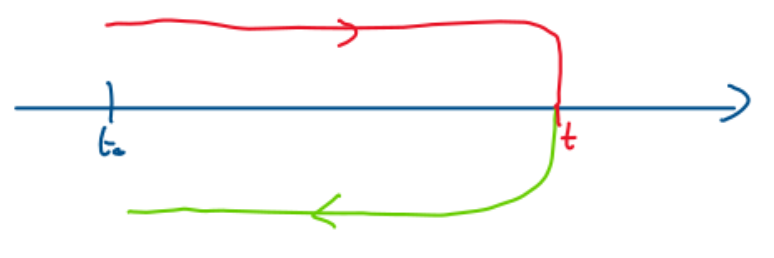
\includegraphics[width=0.82\linewidth]{Pictures/Gell-Mann_Timeordering_Problem.png}
  \caption{Skizze der Zeitentwicklung entlang der Kontur: der obere Ast ist zeitgeordnet und beschreibt die Entwicklung von $t_0$ nach $t$, der linke Ast ist antizeitgeordnet und fuehrt von $t$ wieder nach $t_0$.}
  \label{fig:gell-mann-low-kontur}
\end{figure}

Die Anwendung quantenfeldtheoretischer Methoden setzt dabei eine einheitliche Zeitordnung voraus.

$\rightarrow$ Ziel vom Theorem: die antizeitgeordneten Operatoren in zeitgeordnete Operatoren umzuwandeln.

\subsubsection*{zeitgeordnete GF in der WW-Darstellung}

\begin{equation}
  \begin{aligned}
    G(1,1\mkern1mu')
     & = -\frac{i}{\hbar}\erw{\mathcal T[\psi_H(1)\psi_H^\dagger(1\mkern1mu')]}                                        \\
     & = -\frac{i}{\hbar}
    \left\{
    \begin{aligned}
      \erw{\psi_H(1)\psi_H^\dagger(1\mkern1mu')}  & \quad t_1>t_1\mkern1mu', \\
      -\erw{\psi_H^\dagger(1\mkern1mu')\psi_H(1)} & \quad t_1\mkern1mu'> t_1
    \end{aligned}
    \right.                                                                                                            \\
     & = -\frac{i}{\hbar}
    \left\{
    \begin{aligned}
      \erw{S(t_0,t_1)\psi_0(1) S(t_1,t_0)S(t_1,t_1\mkern1mu') \psi_0^\dagger(1\mkern1mu') S(t_1\mkern1mu',t_0)}  & \quad t_1>t_1\mkern1mu', \\
      -\erw{S(t_0,t_1\mkern1mu')\psi_0^\dagger(1\mkern1mu') S(t_1\mkern1mu',t_0)S(t_0,t_1) \psi_0(1) S(t_1,t_0)} & \quad t_1\mkern1mu'>t_1
    \end{aligned}
    \right.                                                                                                            \\
     & = -\frac{i}{\hbar}
    \left\{
    \begin{aligned}
      \erw{S(t_0,\infty)S(\infty,t_1) \psi_0(1) S(t_1,t_1\mkern1mu') \psi_0^\dagger(1\mkern1mu') S(t_1\mkern1mu',t_0)}  & \quad t_1>t_1\mkern1mu', \\
      -\erw{S(t_0,\infty)S(\infty,t_1\mkern1mu') \psi_0^\dagger(1\mkern1mu') S(t_1\mkern1mu',t_1) \psi_0(1) S(t_1,t_0)} & \quad t_1\mkern1mu'>t_1
    \end{aligned}
    \right.                                                                                                            \\
     & = -\frac{i}{\hbar}\erw{S(t_0,\infty)\,\mathcal T\left[S(\infty,t_0)\psi_0(1)\psi_0^\dagger(1\mkern1mu')\right]}
  \end{aligned}
\end{equation}

Der Zeitordnungsoperator spaltet $S(\infty,t_0)$ auf und stellt die Zeitordnung in der rechten Seite her. Links vom T
ist es antizeitgeordnet. Das versuchen wir jetzt loszuwerden.

\clearpage
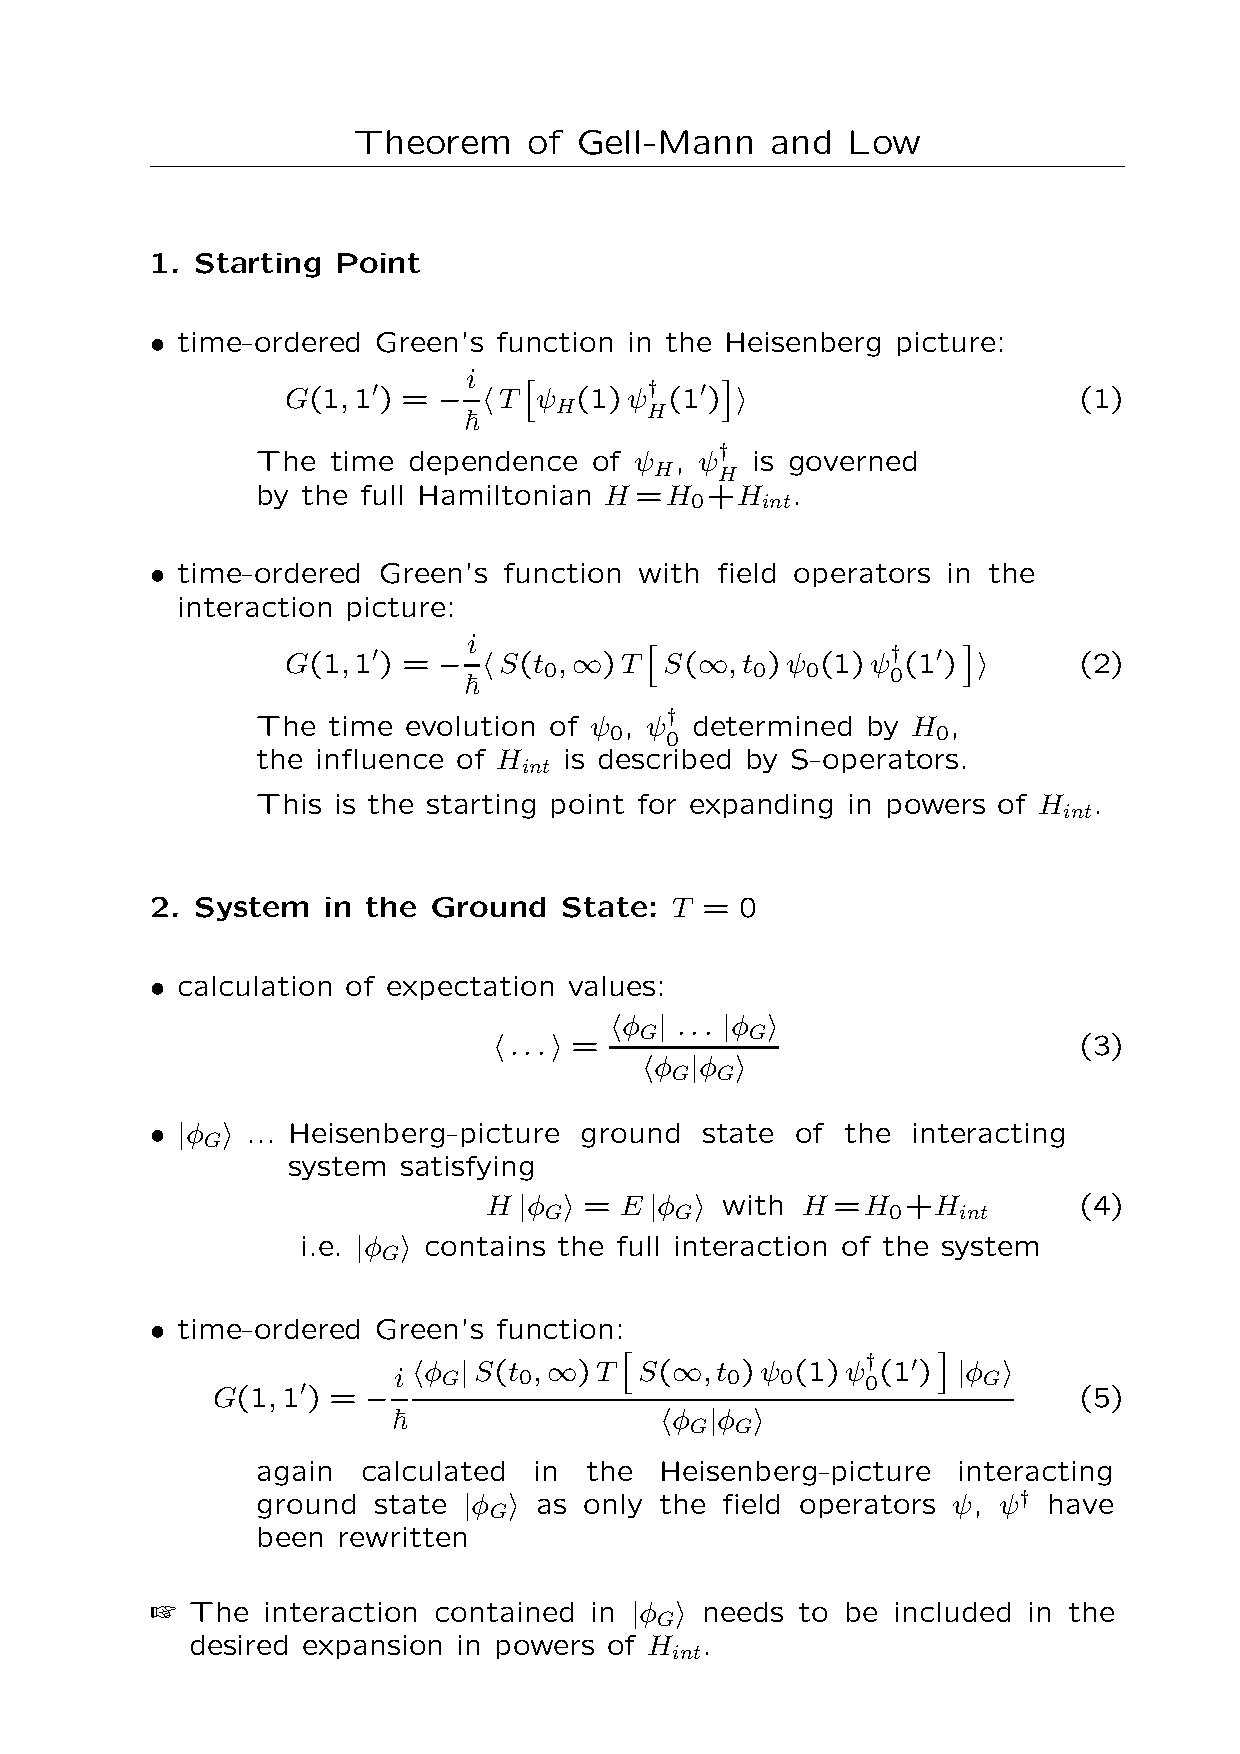
\includepdf[pages=1-3,pagecommand={},fitpaper=true]{PDF/Theorem_von_Gell-Mann_and_Low.pdf}
\clearpage
\subsubsection*{Anmerkungen/Notizen meinerseits}
\begin{itemize}
  \item Was wir mehr oder weniger gemacht haben ist die antizeitgeordneten Operatoren in zeitgeordnete Operatoren umzuwandeln,
        indem wir sie in den Nenner geschrieben haben.
\end{itemize}

\lend{Vorl. 27.04.2026}
\subsection{Entwicklung nach Potenzen der WW}

Da die Wechselwirkung nur noch in $S$ auftritt, ist eine Entwicklung nach Potenzen der Wechselwirkung möglich.
\begin{equation}
  e^{x} = \sum_{n=0}^{\infty} \frac{x^{n}}{n!}
\end{equation}
Setzen wir dies in $S$ ein, so ergibt sich:
\begin{equation}
  \begin{aligned}
    S & = \sum_{n=0}^{\infty} \frac{1}{n!}\left(-\frac{i}{\hbar}\right)^{n} \int_{-\infty}^{\infty} d\bar t_{1}\;\ldots\;\int_{-\infty}^{\infty} d\bar t_{n} \\
      & \qquad\times\; \mathcal{T}\left\{H_{\mathrm{int}}^{0}(\bar t_{1})\ldots H_{\mathrm{int}}^{0}(\bar t_{n})\right\}
  \end{aligned}
\end{equation}
Für die gestörte Greensfunktion folgt damit (mit den neuen Zeitvariablen $\bar t_{1},\ldots,\bar t_{n}$):
\begin{equation}
  \begin{aligned}
    G(1,1\mkern1mu') & = -\frac{i}{\hbar}\frac{1}{\erw{S}}\sum_{n=0}^{\infty} \frac{1}{n!}\left(-\frac{i}{\hbar}\right)^{n}                                                                                                                       \\
                     & \qquad\times\int_{-\infty}^{\infty} d\bar t_{1}\cdots d\bar t_{n}\;\erw{\mathcal{T}H_{\mathrm{int}}^{0}(\bar t_{1})\ldots H_{\mathrm{int}}^{0}(\bar t_{n})\,\psi_{0}(1)\,\psi_{0}^{\dagger}(1\mkern1mu')}                  \\
    \erw{S}          & = \sum_{n=0}^{\infty} \frac{1}{n!}\left(-\frac{i}{\hbar}\right)^{n} \int_{-\infty}^{\infty} d\bar t_{1}\cdots d\bar t_{n}\;\erw{\mathcal{T}\{H_{\mathrm{int}}^{0}(\bar t_{1})\ldots H_{\mathrm{int}}^{0}(\bar t_{n})\}}\,.
  \end{aligned}
\end{equation}
In $H_{\mathrm{int}}^{0}(t)$ treten in der Wechselwirkungsdarstellung Feldoperatoren $\psi_{0}$ und $\psi_{0}^{\dagger}$ auf. Daher führt die Potenzreihenentwicklung von $S$ zu einer Summe von Erwartungswerten mit wachsender Anzahl von Feldoperatoren $\psi_{0}$ und $\psi_{0}^{\dagger}$. Wird später durch das Wick-Theorem vereinfacht.


\subsection{Coulomb-WW als Beispiel}
\stp{Heisenberg-Bild:}
\begin{equation}
  H_{\mathrm{int}}^{H}=\frac{1}{2}\int d^{3}r\int d^{3}r\mkern1mu'\,\psi_{H}^{\dagger}(\vec r,t)\,\psi_{H}^{\dagger}(\vec r\mkern3mu',t)\,V(\vec r-\vec r\mkern3mu')\,\psi_{H}(\vec r\mkern3mu',t)\,\psi_{H}(\vec r,t)
\end{equation}

\stp{Wechselwirkungsbild:}
\begin{equation}
  \begin{aligned}
    \psi_{H}(\vec r,t)           & =S^{\dagger}(t,t_{0})\,\psi_{0}(\vec r,t)\,S(t,t_{0})           \\
    \psi_{H}^{\dagger}(\vec r,t) & =S^{\dagger}(t,t_{0})\,\psi_{0}^{\dagger}(\vec r,t)\,S(t,t_{0})
  \end{aligned}
\end{equation}
Damit folgt
\begin{equation}
  \begin{aligned}
    H_{\mathrm{int}}^{H}(t)   & =S^{\dagger}(t,t_{0})\,H_{\mathrm{int}}^{0}(t)\,S(t,t_{0})                                                                                                                                       \\
    H_{\mathrm{int}}^{(0)}(t) & =\frac{1}{2}\int d^{3}r\int d^{3}r\mkern1mu'\,\psi_{0}^{\dagger}(\vec r,t)\,\psi_{0}^{\dagger}(\vec r\mkern3mu',t)\,V(\vec r-\vec r\mkern3mu')\,\psi_{0}(\vec r\mkern3mu',t)\,\psi_{0}(\vec r,t)
  \end{aligned}
\end{equation}
Fuer das Coulomb-Potential verwenden wir
\begin{equation}
  V(\vec r-\vec r\mkern3mu')=\frac{e^{2}}{4\pi\varepsilon_{0}}\frac{1}{\lvert\vec r-\vec r\mkern3mu'\rvert}
\end{equation}
und in kompakter Schreibweise
\begin{equation}
  V(1-1\mkern1mu')=V(\vec r_{1}-\vec r_{1\mkern3mu'})\,\delta(t_{1}-t_{1\mkern1mu'})
\end{equation}

Fuer die Stoerungsentwicklung von $S$ wird benoetigt:
\begin{equation}
  \int dt\,H_{\mathrm{int}}^{0}(t)=\frac{1}{2}\int d1\int d1\mkern1mu'\,\psi_{0}^{\dagger}(1)\,\psi_{0}^{\dagger}(1\mkern1mu')\,V(1-1\mkern1mu')\,\psi_{0}(1\mkern1mu')\,\psi_{0}(1)
\end{equation}
Entwicklung von $G(1,1\mkern3mu')$ nach Potenzen der WW:
\begin{equation}\label{f:entw_G(1,1')}
  \begin{aligned}
    G(1,1\mkern1mu')       & =G^{(0)}(1,1\mkern1mu')+G^{(1)}(1,1\mkern1mu')+G^{(2)}(1,1\mkern1mu')+\ldots                                                                                              \\
    G^{(0)}(1,1\mkern1mu') & =-\frac{i}{\hbar}\frac{1}{\erw{S}}\erw{\mathcal T\left\{\psi_{0}(1)\psi_{0}^{\dagger}(1\mkern1mu')\right\}}                                                               \\
    G^{(1)}(1,1\mkern1mu') & =-\frac{i}{\hbar}\frac{1}{\erw{S}}\int d\bar t_{1}\,\erw{\mathcal T\left\{\psi_{0}(1)\psi_{0}^{\dagger}(1\mkern1mu')H_{\mathrm{int}}^{0}(\bar t_{1})\right\}}             \\
                           & =\left(-\frac{i}{\hbar}\right)^{2}\frac{1}{\erw{S}}\frac{1}{2}\int d2\int d2\mkern1mu'\,V(2-2\mkern1mu')                                                                  \\
                           & \quad\times\erw{\mathcal T\left\{\psi_{0}(1)\psi_{0}^{\dagger}(1\mkern1mu')\psi_{0}^{\dagger}(2)\psi_{0}^{\dagger}(2\mkern1mu')\psi_{0}(2\mkern1mu')\psi_{0}(2)\right\}}.
  \end{aligned}
\end{equation}

Das sind also viele Feldoperatoren, die wir mit Hilfe von Wick's Theorem in Produkte von $G^{(0)}$-Funktion umschreiben koennen. Zudem ist anzumerken, dass die Menge an Thermen immer größer wird, für ein genaues Ergebnis allerdings unendlich viele Terme notwendig sind.
\clearpage %hier fand ich dass es schöner aussah
\subsection{Wick-Theorem}

\begin{itemize}
  \item Beachte: Erwartungswert ist imernoch im ww-freien Grundzustand
  \item $\psi_0, \psi_0^\dagger$ nur Zeitentwicklung gemäß H 0\\
        $\rightarrow$ Die Berechnung des Erwartungswertes analog zu freien Teilchen
  \item Wick-Theorem: Operator Identität und damit exakt
\end{itemize}

\begin{center}
  \fbox{%
    \begin{minipage}{0.95\linewidth}
      \raggedright
      \setlength{\parindent}{0pt}
      \setlength{\parskip}{0.8\baselineskip}

      Der Erwartungswert eines Produktes einer beliebigen (geraden) Anzahl von Feldoperatoren $\psi_0$ und $\psi_0^\dagger$ in der Wechselwirkungsdarstellung ist gleich der Summe der Produkte aller möglichen paarweise Erwartungswerte (Kontraktionen) dieser Operatoren.

      In jedem Operatorpaar stehen die Operatoren in der gleichen Reihenfolge, wie im ursprünglichen Erwartungswert.

      Das Vorzeichen eines jeden Summanden ist $(-1)^P$, wobei $P$ die Anzahl der notwendigen Vertauschungen ist, um die Operatoren nebeneinander zu bringen.

      Von Null verschieden sind nur die Kontraktionen mit $\psi$ und $\psi^\dagger$. (Im diagonalen Matrixelement müssen Teilchen, die durch $\psi^\dagger$ erzeugt werden, durch $\psi$ wieder vernichtet werden, und umgekehrt.)

      Die Anwendung des Wick-Theorems ergibt Produkte von Erwartungswerten paarweise zeitgeordneter Feldoperatoren $\psi$ und $\psi^\dagger$, also Greensche Funktionen freier Teilchen.

      Siehe auch: StudIP 07\_Wick-Theorem.pdf\\
      G.C. Wick, \textit{Phys. Rev.} 80, 268 (1950)\\
      Fetter and Walecka, \textit{Quantum Theory of Many-Particle Systems}
    \end{minipage}%
  }
\end{center}

Das Wick-Theorem liefert Produkte von zeitgeordneten Erwartungswerten:
\begin{align}
  G^{(0)}(1,1\mkern1mu')
   & = -\frac{i}{\hbar}\,\erw{T\!\left[\psi_0(1)\,\psi_0^\dagger(1\mkern1mu')\right]}
  \quad \text{(freie GF)}
\end{align}
\begin{equation}
  \begin{aligned}
    G^{(1)}(1,2)
     & = \erw{T\!\left[\psi_0(1)\,\psi_0^\dagger(2)\,\psi_0^\dagger(3)\,\psi_0^\dagger(4)\psi_0(4)\,\psi_0(3)\right]}\,V(3-4) \\
     & = (i\hbar)^3\Big\{
    G_0(1,2)\Big[
              \underbrace{G_0(3,3_+)G_0(4,4_+)}_{\textcolor{red}{\text{a)}}}
              -
              \underbrace{G_0(3,4)G_0(4,3)}_{\textcolor{red}{\text{b)}}}
              \Big]                                                   \\
     & \qquad\;
    - G_0(1,3)\Big[
                \underbrace{G_0(4,4_+)G_0(3,2)}_{\textcolor{red}{\text{c)}}}
                -
                \underbrace{G_0(3,4)G_0(4,2)}_{\textcolor{red}{\text{d)}}}
                \Big]                                                   \\
     & \qquad\;
    - G_0(1,4)\Big[
                \underbrace{G_0(3,3_+)G_0(4,2)}_{\textcolor{red}{\text{c)}}}
                -
                \underbrace{G_0(4,3)G_0(3,2)}_{\textcolor{red}{\text{d)}}}
                \Big]
    \Big\}\,V(3-4)\,.
  \end{aligned}
\end{equation}
Folgende Anmerkungen fürs Verständnis:
\begin{itemize}
  \item Variablen 1, 1', 2, 2' wurden hier der Einfachheit halber in 1, 2, 3, 4 umbenannt
  \item Genau genommen sind es keine Gleichungen da $G^{(1)}(1,1\mkern1mu')$ in \autoref{f:entw_G(1,1')} angegebn ist
  \item Der erste Gleichheitsschritt ist somit einfach nur das Anwenden des Wick-Theorems auf die Erwartungswerte von sechs Operatoren
\end{itemize}

\subsubsection*{Feynman-Diagramm}

% --- Kurze Legende für Diagramme ---
\paragraph{Diagramm-Legende}
Jedem Summanden wird ein spezielles Diagramm zugeordnet (Punkte, Linien, Wellenlinien):
\begin{itemize}
  \item Punkt (Variablen-Satz 1 = $r_1,t_1,s_1$) wird einem Punkt zugeordnet: \icon{dot.png}
  \item Durchgezogene Linie is die freie GF: $G_0(1,1\mkern1mu')$ \icon{line.png}\\
        $\rightarrow$ Für gleiche Argumente $G_0(1,1)$: \icon[6ex]{circle.png}
  \item Wellenlinie: Wechselwirkung $V$ \icon[2.2ex]{wave.png}
  \item Über alle inneren Punkte wird integriert (Summen/Integrale an den Symbolen zuordnen)
\end{itemize}
\begin{figure}[ht]
  \centering
  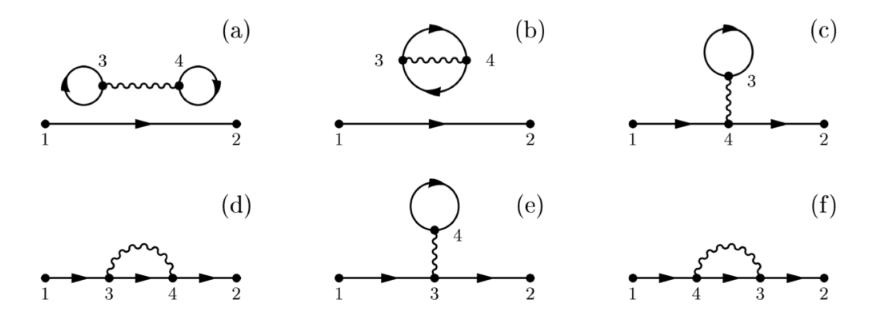
\includegraphics[width=0.8\textwidth]{Pictures/Feynman_for_Coulomb.png}
  \caption{Feynman-Diagramme für die Terme a) bis f) in der Entwicklung von $G^{(1)}(1,2)$.}
  \label{fig:Feynman_Diagramm}
\end{figure}

\lend{Vorl. 04.05.2026}

\subsubsection*{Entwicklung in erster Ordnung der WW}

\begin{itemize}
  \item Zunächst 6 Diagramme
  \item 2 Typen von Diagrammen
        \begin{itemize}
          \item Verbunddiagramme: c--f
          \item Diagramme mit separaten Schleifen: a, b
        \end{itemize}
  \item Unverbundene Anteile entstehen, wenn einige zu $H^{(0)}_{\text{int}}$ gehörende Operatoren untereinander kontrahieren, aber nicht mit $\psi_0(1)\psi_0^\dagger(2)$
  \item Solche Summanden sind in $n$-ter Ordnung gegeben durch:
\end{itemize}

\begin{equation}
  \begin{aligned}
    G^{(n)}(1,2)
     & = \frac{-i}{\hbar}\frac{1}{\erw{S}}\frac{1}{n!}\left(\frac{-i}{\hbar}\right)^n
    \int\!\mathrm{d}\bar{t}_1\cdots\!\int\!\mathrm{d}\bar{t}_m\,
    \erw{T\!\left[\psi_0(1)\,\psi_0^\dagger(2)\,H^{(0)}_{\text{int}}(\bar{t}_1)\cdots H^{(0)}_{\text{int}}(\bar{t}_m)\right]} \\
     & \quad\cdot
    \underbrace{\frac{n!}{m!(n-m)!}}_{\shortstack{Zahl der Möglichkeiten\\die $n$ Operatoren in \\zwei Gruppen aufzuteilen}}
    \int\!\mathrm{d}\bar{t}_{m+1}\cdots\!\int\!\mathrm{d}\bar{t}_n\,
    \erw{T\!\left[H^{(0)}_{\text{int}}(\bar{t}_{m_1+1})\cdots H^{(0)}_{\text{int}}(\bar{t}_n)\right]}
  \end{aligned}
\end{equation}

\begin{itemize}
  \item Zu einem Verbunddiagramm in einer bestimmten Ordnung kommen in den folgenden Ordnungen alle möglichen unverbundenen Anteile hinzu.
        \begin{itemize}
          \item Zu allen Diagrammen in \autoref{fig:Feynman_Diagramm} kommen in zweiter Ordnung die unverbundenen Anteile von a) und b) hinzu.
          \item Theoretisch kann in zweiter Ordnung alle Diagramme aus erster Ordnung mit dem unverbundenen Anteil kombiniert werden der von 1 $\to$ 2 geht.
        \end{itemize}
  \item Zu den Verbunddiagrammen $n$-ter Ordnung addieren sich in den folgenden Ordnungen alle Diagramme, die dieses Verbunddiagramm und zusätzlich unverbundene Anteile enthalten.
\end{itemize}

\begin{equation}
  \begin{aligned}
    G^{(n)}(1,2)
     & = \frac{-i}{\hbar}\frac{1}{\erw{S}}\frac{1}{m!}\left(\frac{-i}{\hbar}\right)^m
    \int\!\mathrm{d}\bar{t}_1\cdots\!\int\!\mathrm{d}\bar{t}_m\,
    \erw{T\!\left[\psi_0(1)\,\psi_0^\dagger(2)\,H^{(0)}_{\text{int}}(\bar{t}_1)\cdots H^{(0)}_{\text{int}}(\bar{t}_m)\right]}   \\
     & \underbrace{\quad\cdot \sum\limits_{n=m}^{\infty}\!
         \frac{1}{(n-m)!} \left(\frac{-i}{\hbar}\right)^{n-m} \int\!\mathrm{d}\bar{t}_{m_1+1}\cdots\!\int\!\mathrm{d}\bar{t}_n\,
         \erw{T\!\left[H^{(0)}_{\text{int}}(\bar{t}_{m_1+1})\cdots H^{(0)}_{\text{int}}(\bar{t}_n)\right]}}_{\erw{S}}
  \end{aligned}
\end{equation}

$\Rightarrow$ In der Störungsreihe der GF kürzt sich der Vorfaktor $\frac{1}{\erw{S}}$ gerade gegen die Beiträge der unverbundenen Diagramme weg\\
$\qquad \hookrightarrow$ Das Kürzen funktioniert nur, wenn man unendlich viele Summanden also Ordnungen hat
\begin{itemize}
  \item Zur weiteren Vereinfachung: Zsf. Von Diagrammen bzw. Summandem, die sich nur in der Bezeichnung unterscheiden
        \begin{itemize}
          \item n-te Ordnung entstehen n Linien der WW \icon[2.5ex]{wave.png}
          \item  n! äquivalente Diagramme durch Permutieren aller n Paar (1,1') $\to$ Vertauschung der Verbindung $\Rightarrow$ 1/n! kürzen
          \item 2$^n$ äquivalente Diagramme durch Vertauschen von 1 und 1' an einer WW $\Rightarrow$ 1/2 kürzen
        \end{itemize}
  \item Bei anderen WW als Coulomb kürzen sich Terme maybe nicht; WW haben im allg. aber nicht mehr als vier Operatoren
\end{itemize}

\subsubsection*{Zusammenfassung der Störungsentwicklung von G(1,2)}

\begin{equation}
  \begin{aligned}
    G(1,2)                                                                      & = G^{(0)}(1,2)                                 & \qquad \text{0.Ordnung} \\
                                                                                & + i\hbar\int\!\mathrm{d}3\!\int\!\mathrm{d}4\,
    \left[ G_0(1,3)G_0(3,4)G_0(4,2) - G_0(1,3)G_0(4,4)G_0(4,2) \right]   V(3-4) & \qquad \text{1.Ordnung}                                                  \\
  \end{aligned}
\end{equation}

\begin{figure}[ht]
  \centering
  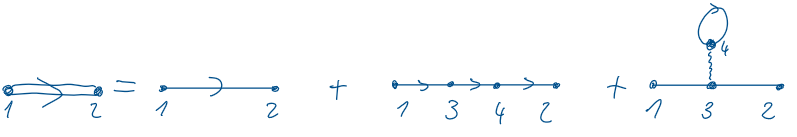
\includegraphics[width=0.8\textwidth]{Pictures/chem_feynman_1Ordnung.png}
  \caption{Chematische Darstellung der Feynman-Diagramme für die Störungsentwicklung von $G(1,2)$ bis zur ersten Ordnung. Alle doppelten bzw. unnötigen wurden direkt rausgekürzt. Dadurch Fallen die Terme $1/n!$ und $1/2$ weg. Allgemein ist mit der Wellenlinie immer $i\hbar V$ gemeint. Deswegen fehlt der Term in dem Bild.}
  \label{fig:chem_feynman_1ord}
\end{figure}

\lend{Vorl. 08.05.2026 }
\addcontentsline{toc}{subsection}{Regeln für die Diagramm Technik}
\includepdf[
  pages=1,
  fitpaper=true,
  pagecommand={%
      \begin{tikzpicture}[remember picture,overlay]
        \node[anchor=north, xshift=-5.0cm, yshift=-1.2cm] at (current page.north) {\Large\bfseries\textcolor{red}{2.6 }};
        \node[anchor=north west, align=left, text width=16cm, xshift=3.5cm, yshift=-3.6cm] at (current page.north west) {\small $\rightarrow$ Als Folgerung aus der Störungsentwicklung in Potenzen der WW und dem Wick-Theorem.};
      \end{tikzpicture}%
    }
]{PDF/10_Regeln_für_die_Konstruktion_von_Diagrammen.pdf}
\clearpage
\subsection{Einführung von Bloch-Diagrammen}
\subsubsection*{Selbstenergie-Blöcke und Dyson-Gleichung}

\stp{In der Mehrheit der quantenstatistischen Probleme ist es nicht möglich, sich auf die ersten Terme der Störungsreihe zu beschränken.}

\stp{Selbstenergie-Blöcke: Betrachten alle Diagramme, die nicht aus zwei oder mehreren Teilen bestehen, die nur durch eine $G$-Linie verbunden sind.}\\
$\hookrightarrow$ z.B. beide Diagramme in 1. Ordnung und $e-j$ in 2. Ordnung

\stp{Diese inneren Anteile haben folgende Struktur:}
\begin{figure}[ht]
  \centering
  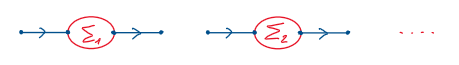
\includegraphics[width=0.5\textwidth]{temp_diagrams/11_05_diagrams/img1_modules.png}
  \label{fig:Selbstenergie_Block}
\end{figure}
\stp{Die Summe aller Selbstenergie-Blöcke ist die Selbstenergie:}
\begin{equation}
  \Sigma(1,2) = \sum\limits_i \Sigma_i(1,2)
\end{equation}
\stp{Die Gesamtheit aller Diagramme lässt sich darstellen als:}
\begin{figure}[ht]
  \centering
  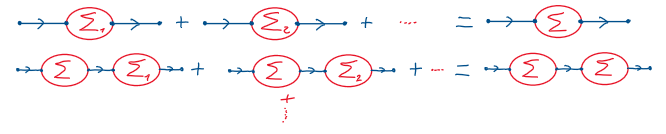
\includegraphics[width=0.6\textwidth]{temp_diagrams/11_05_diagrams/img2_comb_modules.png}
  \label{fig:Selbstenergie_Bloecke}
\end{figure}
\begin{equation}
  \begin{aligned}
    G & = G_0 + G_0 \Sigma(G_0 + G_0 \Sigma G_0 + G_0 \Sigma G_0 \Sigma G_0 + \ldots) \\
      & = G_0 + G_0 \Sigma G
  \end{aligned}
\end{equation}
\stp{Mit Argumenten und Integral über innere Punkte ergibt sich die \textbf{Dyson-Gleichung}:}
\begin{equation}
  \boxed{G(1,2) = G_0(1,2) + \int d3 \, d4 \, G_0(1,3) \Sigma(3,4) G(4,2)}
\end{equation}
\begin{figure}[ht]
  \centering
  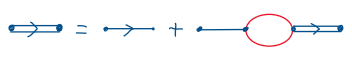
\includegraphics[width=0.4\textwidth]{temp_diagrams/11_05_diagrams/img3_dyson.png}
  \label{fig:Dyson_Gleichung}
\end{figure}
$\Rightarrow$ die rekursive Lösung der Dyson-Gleichung generiert die gesamte Störungsreihe.

\subsubsection*{Polarisationsblöcke}

\stp{Ähnliche Analyse kann für die WW durchgeführt werden:}
Coulomb WW in niedriger Ordnung wird in Diagrammen höherer Ordnung ersetzt durch zwei Coulomb-Linien mit Einschlüssen.
\begin{figure}[ht]
  \centering
  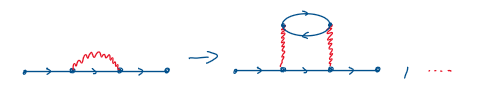
\includegraphics[width=0.55\textwidth]{temp_diagrams/11_05_diagrams/img4_int_progress.png}
  \label{fig:int_progress}
\end{figure}
\begin{figure}[ht]
  \centering
  
\includegraphics[width=0.55\textwidth]{temp_diagrams/11_05_diagrams/img5_int_modules.png}
  \label{fig:int_modules}
\end{figure}
\stp{Definition:}
Die Diagramme, die nicht aus zwei Teilen bestehen, die nur durch eine $v$-Linie verbunden sind \\
$\rightarrow$ die Einschlüsse zwischen zwei Coulomb-Linien sind die \textbf{Polarisationsblöcke}.

\stp{Summe aller Polarisationsblöcke:}
\begin{equation}
  P(\eta) = \sum\limits_i P_i(\eta)
\end{equation}

Durch eine analoge Argumentation wie bei der Selbstenergie erhält man:
\begin{equation}
  \begin{aligned}
    W & = V + VPV + VPVPV + \ldots \\
      & = V + VP(V + VPV)          \\
      & = V + VPW
  \end{aligned}
\end{equation}
\stp{Mit Argumenten und Integrationsvariablen ergibt sich die Dyson-Gleichung für die abgeschirmte WW:}
\begin{equation}
  \boxed{W(1,2) = V(1,2) + \int d3 \, d4 \, u(1,3) P(3,4) W(4,2)}
\end{equation}
Dies ist die \textbf{Bethe-Salpeter-Gleichung für abgeschirmte Coulomb-Wechselwirkung} (Dyson-Gleichung für $W$ statt $U$).

\lend{Vorl. 11.05.2026}[Vorl. 18.05.2026]

\subsubsection*{Vertexblöcke}
Vertexblöcke sind alle irreduziblen Diagrammteile mit genau drei Eckpunkten. Dabei entspricht eine der drei angeschlossenen Linien einer Coulomb-Wechselwirkung $v$, die beiden anderen sind freie Propagatorlinien $G_0$. Solche Blöcke beschreiben also die elementare Kopplung einer WW-Linie an zwei Fermionenlinien.
\begin{figure}[ht]
  \centering
  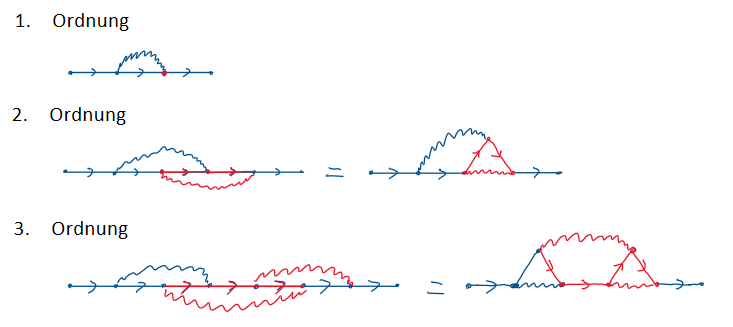
\includegraphics[width=0.75\textwidth]{temp_diagrams/18_05_diagrams/vertexParts.png}
  \label{fig:vertexParts}
\end{figure}\pagebreak
Vertexblöcke werden oft auch mit $\Gamma$ bezeichnet.

\subsubsection*{Aufwertung: Methode zur Bestimmung von $$\Sigma$$ und $$P$$ }
Alle Selbstenergie und Polarisationsdiagramme lassen sich durch Aufwertung der Diagramme niedrigster Ordnung erstellen (wie man sich zeichnerisch vergewissern kann)\\
$\hookrightarrow$ Mit Aufwertung lassen sich alle erstellen, selbstenergie muss man dann raussuchen

\begin{enumerate}
  \item $G_0 \Rightarrow G$ in bisherige $G_0$-Linien alle möglichen Selbstenergie \textbf{beiträge} einschieben
  \item $V \Rightarrow V_s$ in v-Linien alle möglichen Polarisationsblöcke
  \item Einfügen der Vertexbeiträge
\end{enumerate}

\underline{Selbstenergie:}\\
Die Komplette selbstenergie entsteht durch Aufwertung der beiden niedrigsten Selbstenergie-Diagramme
\begin{figure}[ht]
  \centering
  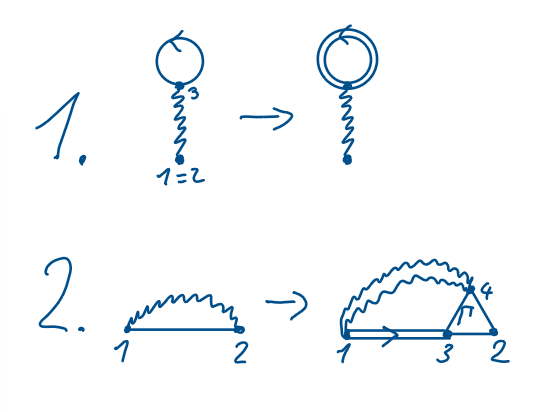
\includegraphics[width=0.4\textwidth]{temp_diagrams/18_05_diagrams/auf_selbstenergie.png}
  \label{fig:auf_selbstenergie}
\end{figure}
Zu 1: man kann sich zeichnerisch davon überzeuge, dass die v-Linie nicht aufgewertet werden darf. Hierdurch würden Beiträge entstehen, die bereits bei $G_0$ Aufwertung geliefert werden.

\underline{Polarisations-blöcke:}\\
Die komplette polarisationsfunktion entsteht durch die Aufwertung des Polarisationsblocks niedrigster Ordnung
\begin{figure}[H]
  \centering
  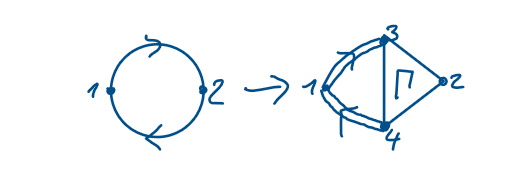
\includegraphics[width=0.4\textwidth]{temp_diagrams/18_05_diagrams/auf_polaristation.png}
  \label{fig:auf_pol}
\end{figure}

\subsubsection*{Zusammenfassung der analytischen Ausdrücke}
\begin{equation}
  \begin{aligned}
    \Sigma(1,2) &= -i\hbar \int d3 \, v(1-2) \, G(3,3^+) \\
                &\quad + i\hbar \int d3 \, d4 \, G(1,3) \, v(1,4) \, \Gamma(3,4,2)
  \end{aligned}
\end{equation}

\begin{equation}
  P(1,2) = i\hbar \int d3 \, d4 \, G(1,3) \, G(4,1) \, \Gamma(3,2,4)
\end{equation}

\noindent niedrigste Näherung für $\Gamma$:
\begin{equation}
  \Gamma_0(1,2,3) = \delta(1-2) \, \delta(1-3)
\end{equation}

\clearpage
\section{Bewegungsgleichung für die Einteilchen GF}
Alternative Methode zur Bestimmung von G

\subsection{Hamiltonian und Heisenberg-Bewegungsgleichung}

\begin{align}
  H & = \sum_{s_1} \int d^3r_1 \, \psi_{s_1}^\dagger(\vec r_1,t_1)\left[-\frac{\hbar^2}{2m}\Delta_{\vec r_1} + U(\vec r_1,t_1)\right]\psi_{s_1}(\vec r_1,t_1) \notag                                     \\
    & \quad + \frac12 \sum_{s_1,s_2} \int d^3r_1 \, d^3r_2, \psi_{s_1}^\dagger(\vec r_1,t_1)\,\psi_{s_2}^\dagger(\vec r_2,t_1)\,V(\vec r_1-\vec r_2)\,\psi_{s_2}(\vec r_2,t_1)\,\psi_{s_1}(\vec r_1,t_1)
\end{align}
Der Hamiltonoperator besteht hier aus dem Einteilchenanteil (kinetische Energie und Gitterpotential/Plasmapotential/etc) und der Coulomb-Wechselwirkung.
\begin{align}
  i\hbar\,\frac{\partial}{\partial t_1} \psi_{s_1}(\vec r_1,t_1)
   & = \bigl[\psi_{s_1}(\vec r_1,t_1),H\bigr] \notag                                                                                              \\
   & = \left[-\frac{\hbar^2}{2m}\Delta_{1} + U(\vec r_1)\right]\psi_{s_1}(\vec r_1,t_1) \notag                                                    \\
   & \quad + \sum_{s_2} \int d^3r_2 \, v(\vec r_1-\vec r_2)\,\psi_{s_2}^\dagger(\vec r_2,t_1)\,\psi_{s_2}(\vec r_2,t_1)\,\psi_{s_1}(\vec r_1,t_1)
\end{align}
Damit erhält man die Bewegungsgleichung für das Feld im Heisenberg-Bild.

\subsubsection*{Zeitableitung der Einteilchen-GF}
\begin{align}
  G(1,1\mkern1mu')
   & = -\frac{i}{\hbar}\,\erw{\mathcal T\!\left[\psi_H(1)\,\psi_H^\dagger(1\mkern1mu')\right]} \notag                                                                                                                                                           \\
   & = \theta(t_1-t_1\mkern1mu')\,\underbrace{G^>(1,1\mkern1mu')}_{-\frac{i}{\hbar}\,\erw{\psi_H(1)\,\psi_H^\dagger(1\mkern1mu')}} + \theta(t_1\mkern1mu'-t_1)\,\underbrace{G^<(1,1\mkern1mu')}_{\frac{i}{\hbar}\,\erw{\psi_H^\dagger(1\mkern1mu')\,\psi_H(1)}}
\end{align}
\begin{align}
  \frac{\partial}{\partial t_1} G(1,1\mkern1mu')
  = \frac{\partial \theta}{\partial t_1}\,G^> + \theta\,\frac{\partial G^>}{\partial t_1} + \frac{\partial \theta'}{\partial t_1}\,G^< + \theta'\,\frac{\partial G^<}{\partial t_1}
\end{align}
Beim Ableiten entstehen also zwei Arten von Termen: Beiträge aus den Theta-Funktionen und Beiträge aus den abgeleiteten GF\@.
\begin{align}
  \frac{\partial}{\partial t_1}\theta(\pm t_1\mp t_1\mkern1mu') & = \pm \delta(t_1-t_1\mkern1mu')
\end{align}
Die Ableitung der Zeitordnung liefert damit direkt den Sprungterm an der gleichen Zeit. Das ist der Ursprung des Antikommutators im nächsten Schritt.
\begin{align}
  i\hbar\,\frac{\partial}{\partial t_1}G(1,1\mkern1mu')
   & = \delta(t_1-t_1\mkern1mu')\,\underbrace{\erw{\psi(1),\psi^\dagger(1\mkern1mu')}+\erw{\psi^\dagger(1\mkern1mu'),\psi(1)}}_{\shortstack[l]{da $t_1=t_1\mkern1mu'$\\$\rightarrow$ Fermiantikommutator\\$=\delta(r_1-r_1\mkern1mu')\delta_{s_1,s_1\mkern1mu'}$}} \notag \\
   & \quad + \erw{\mathcal T\!\left[\bigl(i\hbar\,\frac{\partial}{\partial t_1}\psi(1)\bigr)\,\psi^\dagger(1\mkern1mu')\right]}
\end{align}
Nun setzen wir die Heisenberg-Bewegungsgleichung im zweiten Term ein:
\begin{align}
  i\hbar\,\erw{\mathcal T\!\left[\psi(1)\,\psi^\dagger(1\mkern1mu')\right]}
   & = \left[-\frac{\hbar^2}{2m}\Delta_{1} + U(\vec r_1,t_1)\right]\erw{\mathcal T\!\left[\psi(1)\,\psi^\dagger(1\mkern1mu')\right]}\notag                                                               \\
   & \quad + \sum_{s_2}\int d^3r_2\,v(\vec r_1-\vec r_2)\,\erw{\mathcal T\!\left[\psi_{s_2}^\dagger(\vec r_2,t_1)\,\psi_{s_2}(\vec r_2,t_1)\,\psi_{s_1}(\vec r_1,t_1)\,\psi^\dagger(1\mkern1mu')\right]}
\end{align}
Unter dem Zeitordnungsoperator T lässt der letzte Term wie folgt umformen:
\begin{align}
   & \erw{\mathcal T\!\left[\psi_{s_2}^\dagger(\vec r_2,t_1)\,\psi_{s_2}(\vec r_2,t_1)\,\psi_{s_1}(\vec r_1,t_1)\,\psi^\dagger(1\mkern1mu')\right]}\notag                     \\
   & = \erw{\mathcal T\!\left[\psi_{s_2}(\vec r_2,t_2)\,\psi_{s_1}(\vec r_1,t_1)\,\psi_{s_2}^\dagger(\vec r_2,t_2^+)\,\psi^\dagger(1\mkern1mu')\right]} \qquad t_2=t_1 \notag \\
   & = - \erw{\mathcal T\!\left[\psi(1)\,\psi(2)\,\psi(2^+)\,\psi^\dagger(1\mkern1mu')\right]} \qquad t_2=t_1
\end{align}

\lend{Vorl. 18.05.2026}[Vorl. 22.05.2026]
\newpage
\appendix
\section{Schroedinger-, Heisenberg- und Dirac/Wechselwirkungs-Bild }

In der Quantenmechanik kann dieselbe Physik in verschiedenen Darstellungen formuliert werden. Die am haeufigsten verwendeten sind das Schroedinger-Bild, das Heisenberg-Bild und das Dirac-Bild (Interaction Picture). Sie unterscheiden sich nur darin, welcher Anteil der Zeitentwicklung den Zustaenden bzw. den Operatoren zugeordnet wird. Messbare Groessen sind in allen drei Bildern identisch.

\subsubsection*{Schroedinger-Bild}

Im Schroedinger-Bild tragen die Zustaende die Zeitabhaengigkeit, waehrend Operatoren (sofern sie nicht explizit zeitabhaengig sind) zeitunabhaengig bleiben. Fuer einen Zustand $\ket{\psi_S(t)}$ gilt
\begin{equation}
    i\hbar\,\frac{\partial}{\partial t}\ket{\psi_S(t)}=H\ket{\psi_S(t)}.
\end{equation}
Die Zeitableitung eines Operators ergibt sich nur aus seiner expliziten Zeitabhaengigkeit:
\begin{equation}
    \frac{d}{dt}A_S=\frac{\partial}{\partial t}A_S.
\end{equation}
Ist der Hamiltonoperator zeitunabhaengig, dann ist die Loesung
\begin{equation}
    \ket{\psi_S(t)}=U(t,t_0)\ket{\psi_S(t_0)},
    \qquad
    U(t,t_0)=e^{-\frac{i}{\hbar}H(t-t_0)}.
\end{equation}
Fuer Erwartungswerte folgt
\begin{equation}
    \langle A\rangle_t=\bra{\psi_S(t)}A_S\ket{\psi_S(t)}.
\end{equation}
Setzt man $\ket{\psi_S(t)}=U(t,t_0)\ket{\psi_S(t_0)}$ ein, erhaelt man die direkte Gegenueberstellung von Schroedinger- und Heisenberg-Bild:
\begin{equation}
    \begin{aligned}
        \langle A\rangle_t
         & = \underbrace{\bra{\psi_S(t_0)}U^{\dagger}(t,t_0)}_{\text{Schroedinger: Zustand}}
        \,\underbrace{A_S}_{\text{Operator}}\,
        \underbrace{U(t,t_0)\ket{\psi_S(t_0)}}_{\text{Schroedinger: Zustand}}                \\
         & = \underbrace{\bra{\psi_H}}_{\text{Heisenberg: Zustand}}
        \,\underbrace{\bigl(U^{\dagger}(t,t_0)A_SU(t,t_0)\bigr)}_{\text{Heisenberg: Operator }A_H(t)}\,
        \underbrace{\ket{\psi_H}}_{\text{Heisenberg: Zustand}}.
    \end{aligned}
\end{equation}

\subsubsection*{Heisenberg-Bild}

Im Heisenberg-Bild wird die Zeitentwicklung vollstaendig auf die Operatoren verschoben. Die Zustaende sind (bei zeitunabhaengigem $H$) konstant, z.B.
\begin{equation}
    \ket{\psi_H}=\ket{\psi_S(t_0)}.
\end{equation}
Damit gilt unmittelbar
\begin{equation}
    \frac{d}{dt}\ket{\psi_H}=0.
\end{equation}
Die zugehoerigen Operatoren lauten
\begin{equation}
    A_H(t)=U^{\dagger}(t,t_0)A_SU(t,t_0).
\end{equation}
Fuer zeitunabhaengiges $H$ ist das aequivalent zu
\begin{equation}
    A_H(t)=e^{\frac{i}{\hbar}H(t-t_0)}A_Se^{-\frac{i}{\hbar}H(t-t_0)}.
\end{equation}
Daraus folgt die Heisenberg-Gleichung
\begin{equation}
    i\hbar\,\frac{d}{dt}A_H(t)=\left[A_H(t),H\right]+i\hbar\left(\frac{\partial A_S}{\partial t}\right)_H.
\end{equation}
Fuer Operatoren ohne explizite Zeitabhaengigkeit bleibt nur der Kommutatorterm. Erwartungswerte sind unveraendert:
\begin{equation}
    \langle A\rangle_t=\bra{\psi_H}A_H(t)\ket{\psi_H}.
\end{equation}

\subsubsection*{Dirac-Bild / Interaction Picture}

Das Interaction Picture ist besonders nuetzlich fuer Stoerungstheorie und Feynman-Diagramme. Man zerlegt den Hamiltonoperator in
\begin{equation}
    H=H_0+V,
\end{equation}
wobei $H_0$ der exakt loesbare Teil und $V$ die Wechselwirkung ist. Dann wird die "freie" Dynamik mit $H_0$ auf die Operatoren gelegt, waehrend die zusaetzliche Dynamik durch $V$ in den Zustaenden bleibt:
\begin{equation}
    A_I(t)=e^{\frac{i}{\hbar}H_0(t-t_0)}A_Se^{-\frac{i}{\hbar}H_0(t-t_0)},
\end{equation}
\begin{equation}
    \ket{\psi_I(t)}=e^{\frac{i}{\hbar}H_0(t-t_0)}\ket{\psi_S(t)}.
\end{equation}
Die Zustaende erfuellen damit
\begin{equation}
    i\hbar\,\frac{\partial}{\partial t}\ket{\psi_I(t)}=V_I(t)\ket{\psi_I(t)},
\end{equation}
mit
\begin{equation}
    V_I(t)=e^{\frac{i}{\hbar}H_0(t-t_0)}Ve^{-\frac{i}{\hbar}H_0(t-t_0)}.
\end{equation}
Die zugehoerige Zeitentwicklungsoperatorgleichung lautet
\begin{equation}
    i\hbar\,\frac{\partial}{\partial t}U_I(t,t_0)=V_I(t)U_I(t,t_0),
    \qquad U_I(t_0,t_0)=\mathds{1}.
\end{equation}
Ihre formale Loesung ist die Dyson-Reihe
\begin{equation}
    U_I(t,t_0)=\mathcal{T}\exp\left[-\frac{i}{\hbar}\int_{t_0}^{t}dt'\,V_I(t')\right],
\end{equation}
mit dem Zeitordnungsoperator $\mathcal{T}$. Genau diese Struktur wird in der Vielteilchenphysik fuer Greensche Funktionen und Diagrammtechniken verwendet.

\subsubsection*{Physikalische Einordnung}

Die drei Bilder sind mathematisch aequivalente Beschreibungen derselben Theorie. Das Schroedinger-Bild ist oft der intuitivste Startpunkt. Das Heisenberg-Bild ist fuer Operatorgleichungen und Erhaltungssaetze besonders klar. Das Interaction Picture kombiniert beide Vorteile: freie Ausbreitung steckt in den Operatoren, Wechselwirkungen in den Zustaenden. Deshalb ist es die natuerliche Sprache fuer Streuprozesse, Selbstenergien, renormierte Quasiteilchen und die systematische Entwicklung in Stoerungsordnungen.


\nocite{*}
\bibliographystyle{plain}
\bibliography{myBib}

\end{document}
